%%%%%%%%%%%%%%%%%%%%%%%%%%%%%%%%%%%%%%%%%%%%%%%%%%%%%%%%%%%%%%%%%%%%%%%%%%%%%%%%
%2345678901234567890123456789012345678901234567890123456789012345678901234567890
%        1         2         3         4         5         6         7         8

\documentclass[letterpaper, 10 pt, conference]{ieeeconf}  % Comment this line out
                                                          % if you need a4paper
%\documentclass[a4paper, 10pt, conference]{ieeeconf}      % Use this line for a4
                                                          % paper

\IEEEoverridecommandlockouts                              % This command is only
                                                          % needed if you want to
                                                          % use the \thanks command
\overrideIEEEmargins
% See the \addtolength command later in the file to balance the column lengths
% on the last page of the document



% The following packages can be found on http:\\www.ctan.org
\usepackage{graphics} % for pdf, bitmapped graphics files
\usepackage{epsfig} % for postscript graphics files
\usepackage{mathptmx} % assumes new font selection scheme installed
\usepackage{times} % assumes new font selection scheme installed
\usepackage{amsmath} % assumes amsmath package installed
\usepackage{amssymb}  % assumes amsmath package installed
\usepackage{subfigure}
\usepackage{xcolor}

\newcommand{\usequence}[2]{(u_{i,t})_{i=1,t=1}^{#1,#2}}
\newcommand{\contTilde}[1]{\mathbf{\tilde{#1}}}
\newcommand{\transpose}{\mathsf{T}}
\newcommand{\myinner}[1]{\langle(#1)x,x\rangle}
\newcommand{\quadinner}[1]{x^{\transpose}(#1)x}
\DeclareMathOperator{\contB}{\mathbf{B}}
\DeclareMathOperator{\Log}{\mathrm{Log}}
\newcommand{\BK}[1]{\mathbf{B}\bar{K}_{#1}}
%bound \| x_t - x_{t|t} \|
\newcommand{\boundxtxtgt}[2]{C_{fb}^{2}\|\bar{x}_{1}\|[\frac{C_{K}}{\gamma-1}\bigg(\frac{1-(\eta\gamma)^{#1}}{1-\eta\gamma} - \frac{1-\eta^{#1}}{1-\eta} \bigg){#2}+\varepsilon_{K}\bigg(\frac{(#1-1)\eta^{#1+1}-#1\eta^{#1}+\eta}{(1-\eta)^{2}}\bigg)]}
\DeclareMathOperator{\tempRBP}{R + B^{\transpose}PB}

% \newcommand{\boundxtxtgt1}[1]{\frac{#1}{2}}
%bound |K_t|t - K_t^*|
\newcommand{\boundKt}{C_{K^{'}}\gamma^{W-1} + \gamma_{K^{'}}}

%bound xt|t
\newcommand{\boundxtgt}[1]{C_{fb}\eta^{#1}}

% \newcommand{\\det}{\mathit{\det}}
% \newcommand{\Log}[1]{\text{Log}}

\newtheorem{problem}{Problem}
\newtheorem{lemma}{Lemma}
\newtheorem{assumption}{Assumption}
\newtheorem{definition}{Definition}
\newtheorem{corollary}{Corollary}
\newtheorem{proposition}{Proposition}
\newtheorem{remark}{Remark}
\newtheorem{theorem}{Theorem}

\title{\LARGE \bf
On the Regret Analysis of Online Feedback Potential Dynamic Game via Trajectory Prediction and Tracking
}

%\author{ \parbox{3 in}{\centering Huibert Kwakernaak*
%         \thanks{*Use the $\backslash$thanks command to put information here}\\
%         Faculty of Electrical Engineering, Mathematics and Computer Science\\
%         University of Twente\\
%         7500 AE Enschede, The Netherlands\\
%         {\tt\small h.kwakernaak@autsubmit.com}}
%         \hspace*{ 0.5 in}
%         \parbox{3 in}{ \centering Pradeep Misra**
%         \thanks{**The footnote marks may be inserted manually}\\
%        Department of Electrical Engineering \\
%         Wright State University\\
%         Dayton, OH 45435, USA\\
%         {\tt\small pmisra@cs.wright.edu}}
%}

\author{Yitian Chen, Timothy Molloy, Iman Shames% <-this % stops a space
}


\begin{document}



\maketitle
\thispagestyle{empty}
\pagestyle{empty}


%%%%%%%%%%%%%%%%%%%%%%%%%%%%%%%%%%%%%%%%%%%%%%%%%%%%%%%%%%%%%%%%%%%%%%%%%%%%%%%%
\begin{abstract}
In this paper, we propose and analyse a new method for online feedback potential dynamic game for linear system dynamics and time-varying quadratic costs. The cost matrices are revealed sequentially for each player with the potential for future values to be previewed over a short window. Our novel method involves using the available cost matrices to predict the optimal trajectory, and a tracking controller to drive the system towards it. We adopted the notion of \emph{dynamic social regret} to measure the performance of this proposed method for the online feedback potential dynamic game, with our main result being that the \emph{dynamic social regret} of our method is upper bounded by a constant. Moreover, the regret is upperbounded by a sum of two terms. One decays exponentially as the preview horizon grows, while the other depends on the distance between cost matrices for each player at each time step. In our simulations, we demonstrate that the \emph{dynamic social regret} for our method stabilizes at a constant level as the time horizon grows while also showing a faster-than-exponential decay as the preview window length increases when the time step is fixed.
\end{abstract}


%%%%%%%%%%%%%%%%%%%%%%%%%%%%%%%%%%%%%%%%%%%%%%%%%%%%%%%%%%%%%%%%%%%%%%%%%%%%%%%%
\section{INTRODUCTION}
(\color{red}This part i just put some random stuff on to help us decide how long the introduction should be\color{black})

In the enchanting world of Harry Potter, where magic and mystery seamlessly entwine, we uncover an intriguing intersection with the captivating field of game theory. Imagine a scenario where Harry, Hermione, and Ron, the trio who captured our hearts, find themselves facing a perplexing dilemma. In their relentless quest to thwart the malevolent plans of Lord Voldemort, they often confront situations that demand not only courage and wizardry but also intricate strategic thinking.

Picture this: Harry Potter must decide whether to take the Polyjuice Potion to impersonate a Death Eater, a choice laden with uncertainty and risk. This scenario mirrors the essence of game theory, where individuals must make decisions in the face of uncertain outcomes while considering the potential choices and reactions of others. Much like the characters in J.K. Rowling's magical universe, game theory delves into the intricacies of strategic decision-making, offering profound insights into a myriad of real-world situations.

Game theory, while rooted in mathematics and economics, transcends its academic origins. It embodies the very essence of human interaction, as individuals in both fictional tales and the real world grapple with choices that have ripple effects, sometimes far beyond their initial intentions. Whether it's Harry Potter navigating the complexities of the Triwizard Tournament, Dumbledore orchestrating elaborate schemes, or even the machinations of the Ministry of Magic, the principles of game theory are woven into the fabric of the wizarding world.

Beyond the whimsy of magical spells and fantastical creatures, the Harry Potter saga provides a unique backdrop to explore the multifaceted dimensions of game theory. We will embark on a journey to unravel the enchanting possibilities that arise when the wizarding realm and game theory intersect. Together, we shall decipher the strategic maneuvers, ethical dilemmas, and tactical brilliance that lie beneath the surface of this beloved narrative.

Join us as we navigate the spellbinding universe of potential game theory, where the art of strategic decision-making converges with the enchanting world of Harry Potter, offering insights not only into Hogwarts but also into the complexities of our own reality. Through this exploration, we will unveil the magic of strategic thinking and reveal the hidden connections between the wizarding and academic realms.

\emph{Notation:}
For a matrix $\mathbf{H}$ with 2 rows partitions and 2 column partitions, i.e.,
\begin{align*}
    \mathbf{H} = 
    \begin{bmatrix}
        H_{11} & H_{12}\\
        H_{21} & H_{22}
    \end{bmatrix},
\end{align*}
we define the notation
\begin{equation}
    [\mathbf{H}]_{ij} := H_{ij}(i,j = 1,2).
\end{equation}


Moreover, define the following notation for sequences,
\begin{align}
    &(u_{i,t})_{i=1,t=1}^{2,T-1} := (u_{1,1},u_{2,1},\cdots, u_{1,T-1},u_{2,T-1}),\\
    \begin{split}
         &(u_{i,t})_{i=1,t=1}^{2,\tau-1} \frown (v_{i,t})_{i=1,t=\tau}^{2,T-1}:=(u_{1,1},\cdots,u_{1,\tau-1},v_{1,\tau},\cdots,\\
    &\qquad v_{1,T-1},u_{2,1},\cdots,u_{2,\tau-1},v_{2,\tau},\cdots,v_{2,T-1} ),
    \end{split}
    \end{align}
    For $i=1,2$ and $1\leq t \leq T-1$, define
    \begin{align}
   &R_{t}^{i} := 
   \begin{bmatrix}
       [R_{t}^{i}]_{11} & [R_{t}^{i}]_{12}\\
       [R_{t}^{i}]_{21} & [R_{t}^{i}]_{22}
   \end{bmatrix}\in \mathbb{R}^{2n\times 2n}\text{ with }R_{ij}\in \mathbb{R}^{n\times n},
   \end{align}
   \begin{align}
    &g_{i,t}(x_{t}, \mathbf{u}_{t}) := \frac{1}{2}(x_{t}^{\mathsf{T}}Q_{t}x_{t} + 
    \mathbf{u}_{t}^{\transpose}R_{t}^{i}\mathbf{u}_{t}),
    \end{align}
    and
    \begin{align}
    &g_{i,T}(x) := \frac{1}{2} x^{\mathsf{T}}Q_{T}x,
\end{align}
with $Q_{t}, Q_{T} \in \mathbb{R}^{n\times n}$. $\|\cdot\|$ denotes the 2-norm of a vector or a matrix, depending on its argument. For any symmetric matrices $F,G$ with appropriate dimensions, $F \preceq G$ denotes $G-F$ being positive definite.
Lastly, let $\mathbb{S}_{+}^{n}$ denotes the set of $n$-dimensional square positive semi-definite matrix and $\mathbb{S}_{+}^{n}$ for $n$-dimensional square positive definite matrix, respectively.


\section{PROBLEM FORMULATION}
Consider the discrete-time linear system
\begin{align}
    &x_{t+1} = Ax_{t} + \mathbf{B}\mathbf{u}_{t}\label{eq:linsys},\\
    &x_{1} =\bar{x}_{1}(\bar{x}_1 \in \mathbb{R}^{n})\label{eq:initialx}
\end{align}
for $1\leq t \leq T-1$ with $1\leq T < \infty$ and where $A \in \mathbb{R}^{n\times n}$, $\mathbf{B} = [B^{1}, B^{2}]$, $\mathbf{u}_{t} = [u_{1,t}^{\transpose},u_{2,t}^{\transpose}]^{\transpose}$, $x_{t}\in\mathbb{R}^n$, $u_{i,t} \in \mathbb{R}^{m}$,$B^{i} \in \mathbb{R}^{n\times m}$($i = 1,2$) and $m$ and $n$ are positive integers.


Suppose matrices $Q_{t}$, $[R_{t}^{i}]_{jk}(i,j,k = 1,2)$, $A$ and $B^{i}(i=1,2)$ satisfy the following assumptions,
\begin{assumption}\label{assumption:bounds}
    There exists symmetric positive definite matrices $Q_{min}, Q_{max}, R_{min}, R_{max}$ that
    \begin{equation}
        Q_{min} \preceq Q_{t} \preceq Q_{max},
    \end{equation}
    \begin{equation}
        Q_{t} \in \mathbb{S}^{n}_{++},
    \end{equation}
    for $1\leq t \leq T$, and
    \begin{equation}\label{eq:positiveR}
        R_{min} \preceq 
        \begin{bmatrix}
            [R_{t}^{1}]_{11} & [R_{t}^{1}]_{12}\\
            [R_{t}^{2}]_{21} & [R_{t}^{2}]_{22}
        \end{bmatrix}
        \preceq R_{max},
    \end{equation}
    for $1 \leq t \leq T-1$.
\end{assumption}
\begin{assumption}\label{assumption:controllable}
    Matrix $A$ has full rank, and there exists $\bar{K}$, such that $\rho(A + \contB \bar{K}) < 1$, where $\rho(\cdot)$ denotes the spectral radius operator.
\end{assumption}
\begin{assumption}\label{assumption:lowerQ}
    For any given $t(1\leq t \leq T-1)$, matrices $Q_{t}, R_{t}^{1}, R_{t}^{2}$,
    satisfy
    \begin{equation}
        \lambda_{\min}(Q_{t}) > \max(0,\sigma_{max}(B)\lambda_{min}(\Delta_{R})),
    \end{equation}
    where
    \begin{align*}
        \Delta_{R} := \begin{bmatrix}
            0 & 0\\
            [R_{t}^{2}]_{21} - [R_{t}^{1}]_{21} & [R_{t}^{2}]_{22} - [R_{t}^{1}]_{22}
        \end{bmatrix}.
    \end{align*}
\end{assumption}
The $i$-th player's cost function is then
\begin{equation}\label{eq:LQcost}
    J_{i,T}((x_{t})_{t=1}^{T},(u_{i,t})_{i=1,t=1}^{2,T-1}) := \sum_{t=1}^{T-1} g_{i,t}(x_{t}, \mathbf{u}_{t}) + g_{i,T}(x_{T}).
\end{equation}

Now we can establish the concept of Nash Equilibrium.
The sequence $(x_{t}^{*})_{t=1}^{T},(u_{i,t}^{*})_{i=1,t=1}^{2,T-1}$ is called Feedback Nash Equilibrium, if and only if the following conditions are satisfied. For $1 \leq \tau \leq T$, $(x_{t}^{*\tau})_{t=1}^{T}$ is generated by the sequence of $(u_{i,t})_{i=1,t=1}^{2,\tau-1} \frown (u_{i,t}^{*})_{i=1,t=\tau}^{2,T-1}$, where $u_{i,t}$ is any given control decision for $i = 1,2$ and $1 \leq t \leq \tau-1$. Moreover, $(x_{t}^{(1,\tau)})_{t=1}^{T}$ is generated by $(u_{i,t})_{i=1,t=1}^{2,\tau-1} \frown (u_{1,\tau},u_{2,\tau}^{*}) \frown (u_{i,t}^{*})_{i=1,t=\tau+2}^{2,T-1}$, and similarly to $(x_{t}^{(2,\tau)})_{t=1}^{T}$, which,
% The restrictions on sequence $(x_{t}^{*})_{t=1}^{T},(u_{i,t}^{*})_{i=1,t=1}^{2,T-1}$ is given by the following inequalities,

\begin{equation}\label{eq:nashIneq}
    \begin{split}
        \text{Level T}
        &\begin{cases}
            &J_{1,T}((x_{t}^{*T})_{t=1}^{T}, (u_{i,t})_{i=1,t=1}^{2,T-2} \frown (u_{1,T}^{*},u_{2,T}^{*})) \\ & \leq J_{1,T}((x_{t}^{(1,T)})_{t=1}^{T}, (u_{i,t})_{i=1,t=1}^{2,T-2} \frown (u_{1,T},u_{2,T}^{*})),\\ \\
            &J_{2,T}((x_{t}^{*T})_{t=1}^{T}, (u_{i,t})_{i=1,t=1}^{2,T-2} \frown (u_{1,T}^{*},u_{2,T}^{*})) \\ & \leq J_{2,T}((x_{t}^{(2,T)})_{t=1}^{T}, (u_{i,t})_{i=1,t=1}^{2,T-2} \frown (u_{1,T}^{*},u_{2,T})).
        \end{cases}
    \\ &\qquad \qquad \qquad \vdots \\
    \text{Level 1}
        &\begin{cases}
            &J_{1,T}((x_{t}^{*1})_{t=1}^{T}, (u_{1,1}^{*},u_{2,1}^{*}) \frown (u_{i,t}^{*})_{i=1,t=2}^{2,T-1}) \\ & \leq J_{1,T}((x_{t}^{(1,1)})_{t=1}^{T}, (u_{1,1},u_{2,1}^{*}) \frown (u_{i,t}^{*})_{i=1,t=2}^{2,T-1}),\\ \\
            &J_{2,T}((x_{t}^{*1})_{t=1}^{T}, (u_{1,1}^{*},u_{2,1}^{*}) \frown (u_{i,t}^{*})_{i=1,t=2}^{2,T-1}) \\ & \leq J_{2,T}((x_{t}^{(2,1)})_{t=1}^{T}, (u_{1,1}^{*},u_{2,1}) \frown (u_{i,t}^{*})_{i=1,t=2}^{2,T-1}).
        \end{cases}
    \end{split}
\end{equation}

For convenient use later, we define 
\begin{equation}\label{eq:history}
    \mathcal{H}_{T} := ( \bar{x}_{1},(Q_{t}^{i})_{i=1,t=1}^{2,T},(R_{t}^{i})_{i=1,t=1}^{2,T-1}),
\end{equation}
as the cost matrices available up to time $T$, and
\begin{equation}\label{eq:regret}
 \text{DFLGame}(\mathcal{H}_{T},T):=((x_{t}^{*1})_{t=1}^{T}, (\mathbf{u}_{t}^{*})_{t=1}^{T-1}).
\end{equation}
as an operator that use information $\mathcal{H}_{T}$ to generate Feedback Nash Equilibrium.

For any decisions $(\mathbf{u}_{t})_{t=1}^{T-1}$ and the associated state sequence $(x_{t})_{t=1}^{T}$, we define the \emph{dynamic social regret} as
\begin{equation}
    \begin{split}
        &\text{Regret}_{T}((\mathbf{u}_{t})_{t=1}^{T-1}) := \\
        &\sum_{i=1}^{N} J_{i,T}((x_{t})_{t=1}^{T},(\mathbf{u}_{t})_{t=1}^{T-1}) - J_{i,T}((x_{t}^{*})_{t=1}^{T},(\mathbf{u}_{t}^{*})_{t=1}^{T-1}).
    \end{split}
\end{equation}
Our consideration of \emph{dynamic social regret} is motivated by the concept of dynamic regret from \cite[Equation (5)]{chen_regret_2022} that captures the discrepancy between the performance of a proposed algorithm and the best time-varying policies chosen in hindsight.

The focus of our work is to propose a novel control policy that generates $\mathbf{u}_{t}$ using the information available at time $t$, i.e., $\mathcal{H}_{t}$, and investigate its performance in terms of \emph{dynamic social regret}. We specifically consider the system \eqref{eq:linsys}, with the cost matrices in \eqref{eq:regret} satisfy Assumption \ref{assumption:controllable} for any given $T \geq 1$ and $W < T-1$. At time $1 \leq t \leq T-W-1$, the available information to the players is given by $\mathcal{H}_{t}$ as defined in \eqref{eq:history} and the current state $x_{t}$. It is desired to design a control policies $\pi(\cdot, \cdot)$ of the form \eqref{eq:policy} that yields a bounded \emph{dynamic social regret}, as defined by \eqref{eq:regret}, (\color{red} this part is for justifying what we want to yield from the regret or the algorithm\color{black}).



% consider a feedback control policy $\pi(\cdot,\cdot)$ of the form 
% \begin{equation}\label{eq:policy}
%     \mathbf{u}_{t} = \pi(x_{t}, \mathcal{H}_{t}).
% \end{equation}

% The key contributions of this paper are
% \begin{itemize}
%     \item The proposal of a method to solve an online LQ potential game;
%     \item Development of the dynamic social regret upperbound;
% \end{itemize}



%%%%%%%%%%%%%%%%%%%%%%%%%%%%%%%%%%%%%%%%%%%%%%%%%%%%%%%%%%%%%%%%%%%%%%%%%%%%%%%%
% \section{PROBLEM FORMULATION}
% In this paper, we consider the following problem.
% \begin{problem}[Online Dynamic LQ Game]
     % Consider the system \eqref{eq:linsys}. Let the cost matrices in \eqref{eq:regret} satisfy Assumption \ref{assumption:controllable} for any given $T \geq 1$ and $W < T-1$. At time $1 \leq t \leq T-W-1$, the available information to the players is given by $\mathcal{H}_{t}$ as defined in \eqref{eq:history} and the current state $x_{t}$. It is desired to design a control policies $\pi(\cdot, \cdot)$ of the form \eqref{eq:policy} that yields a regret, as defined by \eqref{eq:regret}, ???.
     % , that is independent of the bounds given in Assumption \ref{assumption:bounds}.
% \end{problem}

\section{Proposed Approach and Regret Analysis}
\paragraph{Prediction. } 
Define 
\begin{equation}
\begin{split}
    \bar{\mathcal{H}}_{t} = (&\bar{x}_{1}, (Q_{\tau})_{\tau=1}^{t+W} \frown(Q_{t+W})_{\tau=t+W+1}^{T},\\
    &(R_{\tau}^{i})_{i=1,\tau=1}^{2,t+W} \frown(R_{t+W}^{i})_{i=1,\tau=t+W+1}^{2,T-1}).
\end{split}
\end{equation}
We predict a trajectory by using the current cost matrices and setting the future unknown cost matrices to be equal to the known value at time $t+W$, i.e.,
\begin{equation}
    ((x_{\tau|t})_{\tau=1}^{T},(\mathbf{u}_{\tau|t})_{\tau=1}^{T-1}) = \text{DFLGame}(\bar{\mathcal{H}}_{t},T).
\end{equation}

\paragraph{Prediction Tracking. } We propose the following feedback control policy
\begin{equation}\label{eq:policy}
    \pi(x_{t},\mathcal{H}_{t}) := \bar{K}(x_{t}-x_{t|t}) + \mathbf{u}_{t|t},
\end{equation}
where $\bar{K}\in \mathbb{R}^{m\times n}$ is a control matrix such that $\rho(A+\mathbf{B}\bar{K}) < 1$, and $\rho(\cdot)$ denotes the matrix spectral radius.


\subsection{Regret Analysis}
Consider the linear system defined by \eqref{eq:linsys}. For a given time horizon $T \geq 1$ and preview window length $0 \leq W \leq T-1$. Suppose that at time $1\leq t \leq T-1$ the control input $u_{t}$ is generated by $\pi(\cdot,\cdot)$ as given by \eqref{eq:policy}. Under Assumption \ref{assumption:bounds}-\ref{assumption:lowerQ}, we introduce the following definitions to establish the concept of Linear quadratic dynamic potential game.
\begin{definition}[LQDFG]\label{def:LQDFG}
    A linear quadratic dynamic feedback game(LQDFG) is, for each player $i(i = 1,2)$ and a given positive integer $T$, suppose $J_{i,t}(\cdot,\cdot)$ for $1\leq t\leq T$ are known by each player, where $J_{i,t}$ is defined at \eqref{eq:LQcost}. At stage $t(1\leq t\leq T-1)$, each player chooses the control $u_{i,t}^{*}$ that satisfies the inequalities given in \eqref{eq:nashIneq}. 
\end{definition}

% Before we introduce the concept of linear quadratic dynamic feedback potential game(LQDFPG), let's start by introducing the following linear quadratic optimal control problem(LQOCP). For a given $T(T\geq 1)$, 
% suppose $\Psi_{t}:\mathbb{R}^{n}\times\mathbb{R}^{m}\rightarrow \mathbb{R}(1\leq t \leq T-1)$ and $\Psi_{T}:\mathbb{R}^{n}\rightarrow \mathbb{R}$ are being continuous and twice continuously differentiable in their arguments.
% Under Assumption \ref{assumption:controllable}, LQOCP is defined by the following problem.

\begin{definition}[LQOCP]\label{def:LQOCP}
    The problem of linear quadratic optimal control problem(LQOCP) is the following.
    Suppose $T$ is a positive integer. For given $(\bar{Q}_{t})_{t=1}^{T},(\bar{R}_{t})_{t=1}^{T-1}$ satisfy Assumption \ref{assumption:bounds}, find $\{\mathbf{u}_{t}\}_{t=1}^{T-1}$ such that
    \begin{equation}\label{eq:LQOCP}
\begin{split}
    \min_{\{\mathbf{u}_{t}\}_{t=1}^{T-1}}& \sum_{t=1}^{T-1} x_{t}^{\transpose}\bar{Q}_{t}x_{t} + \mathbf{u}_{t}^{\transpose}\bar{R}_{t}\mathbf{u}_{t} + x_{T}^{\transpose}\bar{Q}_{T}x_{T}\\
    &\text{\qquad s.t. Equation \eqref{eq:linsys}}.
\end{split}
\end{equation}
\end{definition}
\begin{definition}
    The dynamic game is referred to as a linear quadratic dynamic feedback potential game(LQDFPG), if the solution of a given LQOCP, in feedback form, provides a feedback Nash equilibrium for the linear quadratic dynamic game. 
\end{definition}


\begin{theorem}\label{thm:main}
Consider the linear system defined by \eqref{eq:linsys}. For a given time horizon $T \geq 1$ and preview window length $0 \leq W \leq T-1$. Suppose that at time $1 \leq t \leq T-1$ the control input $u_t$ is generated by policy $\pi(\cdot,\cdot)$ as given by \eqref{eq:policy}. Under Assumption \ref{assumption:bounds}-\ref{assumption:lowerQ}, the regret defined by \eqref{eq:regret} satisfies
    \begin{align*}
        &\text{Regret}_{T}((\mathbf{u}_{t})_{t=1}^{T-1})< \|\bar{x}_{1}\|^{2}\bigg[\Delta_{a}(\gamma^{W},\varepsilon_{K^{'}})\frac{1-q^{2T}}{1-q^{2}}\\
        &+  \Delta_{b}(\gamma^{W},\varepsilon_{K^{'}})\frac{1-\eta^{2T}}{1-\eta^{2}}+ \Delta_{c}(\gamma^{W},\varepsilon_{K^{'}})\frac{1-(q\eta)^{T}}{1-q\eta}\bigg],
    \end{align*}
    where $\bar{P}_{max}$ satisfies
    \begin{align*}
        \bar{P}_{max} &= \bar{Q}_{max} + A^{\transpose}\bar{P}_{max}A \\
        &- A^{\transpose}\bar{P}_{max}\contB(\bar{R}_{max}+\contB^{\transpose}\bar{P}_{max}\contB)^{-1}\contB^{\transpose}\bar{P}_{max}A,
    \end{align*}
    and
    \begin{align*}
        &\alpha_{\tau,t} := \lambda_{max}(A^{\transpose}(\bar{P}_{\tau+1|t}^{-1}+B\bar{R}_{\tau|t}^{-1}B^{\transpose})^{-1}A),\\
        &\beta_{\tau,t} := \lambda_{min}(\bar{Q}_{\tau|t}),\\ 
        &\gamma := \max_{1\leq \tau,t \leq T} \frac{\alpha_{\tau,t}}{\alpha_{\tau,t}+\beta_{\tau,t}},\\
        &q = \rho(A+B\bar{K}) + \varepsilon(0\leq \varepsilon < 1-\rho(A+B\bar{K})),\\
        &\eta = \sqrt{1-\frac{\lambda_{min}(\bar{Q}_{min})}{\lambda_{max}(\bar{P}_{max})}},\\
        &\Delta_{1} := \max_{t} \frac{1}{2}\sum_{i=1}^{2}(R_{t}^{i}+\mathbf{B}^{\transpose}P_{t+1}^{i}\mathbf{B}),\\
        &\Delta_{2} := \max_{t} \sum_{i=1}^{2}\bigg( (R_{t}^{i}+\mathbf{B}^{\transpose}P_{t+1}^{i}\mathbf{B})\bar{K}_{t}^{*}+\mathbf{B}^{\transpose}P_{t+1}^{i}A\bigg),\\
        &\varepsilon_{1} = \max\bigg(1+\frac{\lambda_{max}(Q_{\tau|t}-Q_{\tau|t_{0}})}{\lambda_{min}(\bar{P}_{\tau|t_{0}})},1+\frac{\lambda_{max}(Q_{\tau|t_{0}}-Q_{\tau|t})}{\lambda_{min}(\bar{P}_{\tau|t})}\bigg),\\
        &h := \log(\frac{\lambda_{max}(\bar{P}_{max})}{\lambda_{min}(\bar{Q}_{min})}),\\
        &\varepsilon_{K} =\|\contB\|\frac{\varepsilon_{1}(e^{h}-1)\lambda_{max}(\bar{P}_{max})}{h(1-\gamma)},\\
        &C_{K} = \left\|(\bar{R}_{min}+\contB^{\mathsf{T}}\bar{Q}_{min}\contB)^{-1}\right\|^{2}\left\|\bar{R}_{max}\contB^{\mathsf{T}}\right\|\frac{\lambda_{max}^{2}(\bar{P}_{max})}{\lambda_{min}(\bar{Q}_{min})},\\
        &D_{K} := \frac{C_{K}q\eta(\gamma-1)}{(q-\eta\gamma)(q-\eta)} + \frac{\varepsilon_{K}q\eta}{(q-\eta)^{2}},\\
        &C_{x} := C_{fb}^{2}D_{K},\\
        &\Delta_{a}(z,y) := 2(\Delta_{1}+\Delta_{2})D_{K}(z,y)C_{x}^{2},\\
        &\Delta_{b}(z,y) := 4\Delta_{1}C_{fb}^{2}(C_{K}^{2}z^{2}+y^{2})+2\Delta_{2}(C_{K}z+y),\\
        &\Delta_{c}(z,y) := 2C_{x}C_{fb}\Delta_{2}(C_{K}z+y+D_{K}),\\
    \end{align*}
\end{theorem}

%%%%%%%%%%%%%%%%%%%%%%%%%%%%%%%%%%%%%%%%%%%%%%%%%%%%%%%%%%%%%%%%%%%%%%%%%%%%%%%%
\section{NUMERICAL SIMULATIONS}
In this section, we numerically demonstrate the performance of the proposed algorithm. Consider the following linear system
\begin{equation}
    x_{t+1} = 
    \begin{bmatrix}
        a & 0\\
        0 & 0.9
    \end{bmatrix}
    x_{t} + 
    \begin{bmatrix}
        -b_{1} & -b_{2}\\
        0 & 0
    \end{bmatrix}\mathbf{u}_{t}.
\end{equation}
In the experiments, the preview window length $W$ ranges from 0 to 6 and the time horizon $T$ ranges from 1 to 200. The cost matrices are with the structure of
\begin{equation}
    Q_{t} = 
    \begin{bmatrix}
        l_{t} & -d_{t}\\
        -d_{t} & 0,
    \end{bmatrix}
\end{equation}
\begin{equation}
    R_{t}^{1} = 
    \begin{bmatrix}
        r_{1,t} & 0\\
        0 & 0,
    \end{bmatrix}
\end{equation}
\begin{equation}
    R_{t}^{2} = 
    \begin{bmatrix}
        0 & 0\\
        0 & r_{2,t},
    \end{bmatrix}
\end{equation}
where we assume that $\frac{b_{1}^{2}}{r_{1,t}}=\frac{b_{2}^{2}}{r_{2,t}} = \beta_{t}$. The above parameters and assumption lead to a LQ potential game. Let $x \sim \mathcal{U}[a,b]$ be $x$ uniformly sampled from range $[a,b]$. In our experiment, we sample $\beta_{t} \sim \mathcal{U}[10,110]$, $l_{t} \sim \mathcal{U}[10,110]$ and $d_{t}\sim \mathcal{U}[-110,-10]$. A similar example has been used in \cite[Section V]{prasad_structure_2023}. We repeat the experiment in 30 trials. The plot in Figure \ref{fig:0preview} and \ref{fig:1preview} demonstrates the average \emph{regret} over 30 monte-carlo trials, with preview window lengths 0 and 1, respectively. The average \emph{regret} saturates at about $t=70$ when at 0 preview window length, while the average \emph{regret} saturates at $t = 40$ when preview window length is 1. These plots empirically demonstrate the main result. The plots in Figure \ref{fig:8timehorizon} and \ref{fig:69timehorizon} demonstrate how the log average \emph{regret} varies if preview window length changes with fixed $t=8$ and $t=69$, respectively. The trends depicted from Figure \ref{fig:8timehorizon} and \ref{fig:69timehorizon} show a faster-than-exponential decay as the preview window length grows from 0 to 6, which validates the theoretical upperbound in Theorem \ref{thm:main}.

\begin{figure}
        \label{fig:experiments}
     \centering
     \subfigure[Regret vs. Time Horizon with 0 Preview Window Length]{
         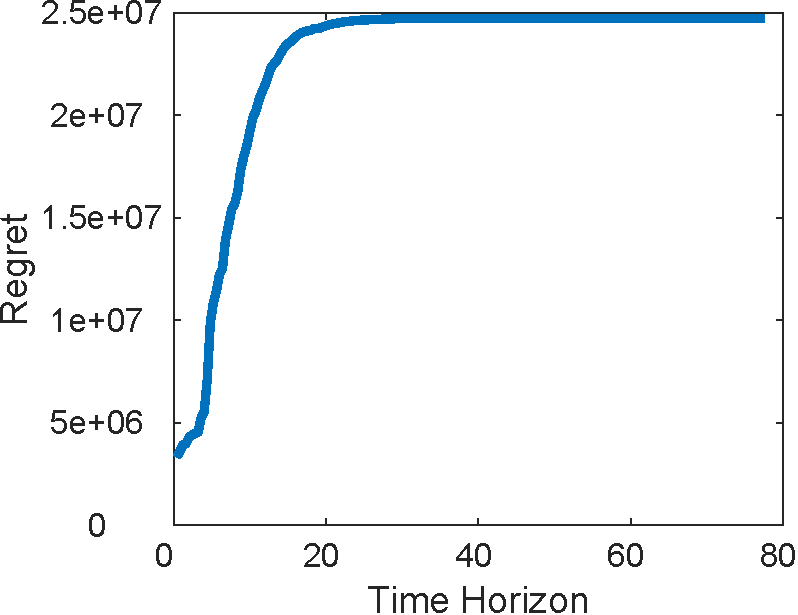
\includegraphics[width=.22\textwidth]{window1.pdf}
    \label{fig:0preview}}
     \subfigure[Regret vs. Time Horizon with 1 Preview Window Length]{
         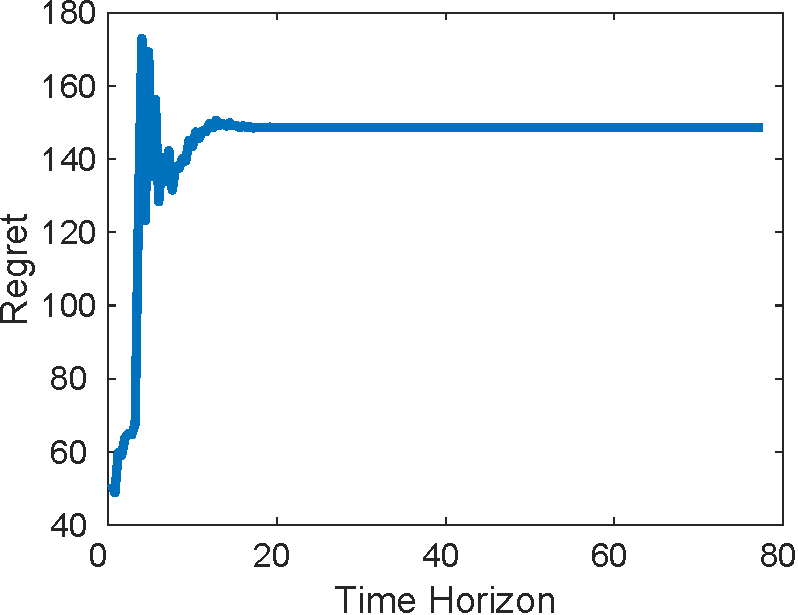
\includegraphics[width=.22\textwidth]{window2.pdf}
    \label{fig:1preview}}
    \\
     \subfigure[Regret vs. Preview Window Length in 8-th Time Horizon]{
         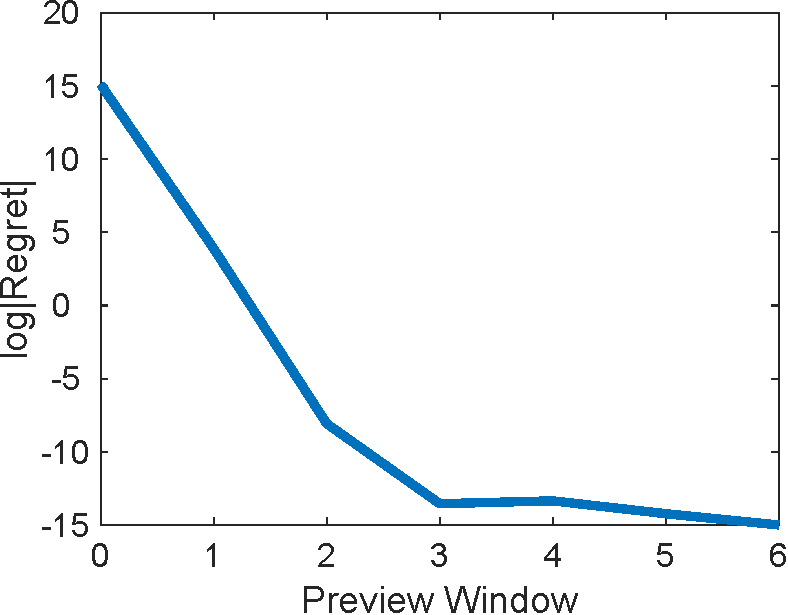
\includegraphics[width=.22\textwidth]{time1.pdf}
    \label{fig:8timehorizon}}
     \subfigure[Regret vs. Preview Window Length in 69-th Time Horizon]{
         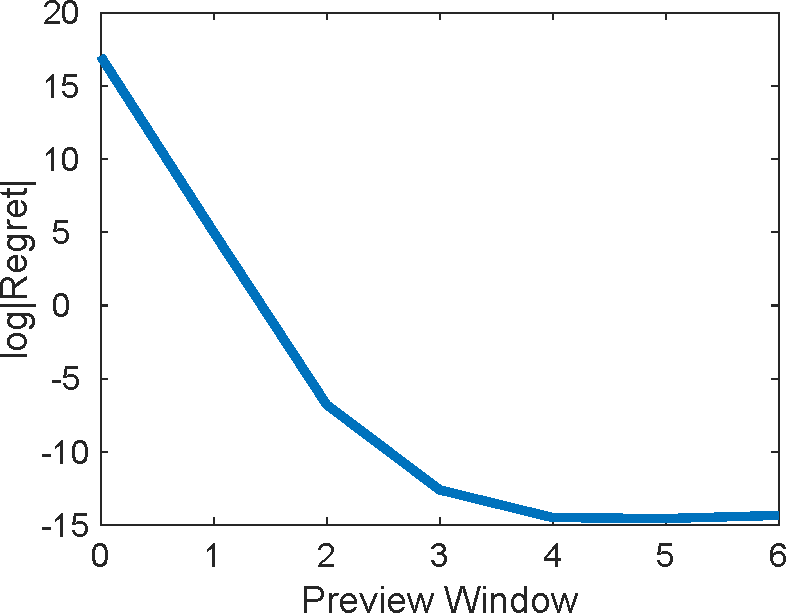
\includegraphics[width=.22\textwidth]{timeThird.pdf}
    \label{fig:69timehorizon}}
    \caption{Performance measure $\text{Regret}_{T}$ for simulated systems.}
\end{figure}

\section{CONCLUSIONS AND FUTURE WORKS}
This paper proposes a novel algorithm for an online feedback potential game, and the analysis of its performance by \emph{dynamic social regret}, which is a natural extension of dynamic \emph{Regret} from \cite[Equation (5)]{chen_regret_2022} suggests that the algorithm yields a sublinear \emph{dynamic social regret}. This paper leads to many interesting research directions which are briefly discussed below. One can investigate the case of $N$-players potential dynamic game with time-varying $A_{t}$ and $\mathbf{B}_{t}$ for the system matrices, then establish new \emph{dynamic social regret} bounds. Another direction could be investigated the case of a zero-sum LQ game that sequentially reveals cost matrices to each player, with removing the assumption of the potential game in the problem setting.


%%%%%%%%%%%%%%%%%%%%%%%%%%%%%%%%%%%%%%%%%%%%%%%%%%%%%%%%%%%%%%%%%%%%%%%%%%%%%%%%
\section{ACKNOWLEDGMENTS}

% The authors gratefully acknowledge the contribution of National Research Organization and reviewers' comments.


%%%%%%%%%%%%%%%%%%%%%%%%%%%%%%%%%%%%%%%%%%%%%%%%%%%%%%%%%%%%%%%%%%%%%%%%%%%%%%%%

\bibliographystyle{plain}
\bibliography{References}
\appendix
\section{Proof of Theorem~\ref{thm:main}}
Before stating the proof of the theorem we introduce the necessary propositions and lemmas.

\begin{lemma}
    For time instant $t$ from $T-1$ to 1, define
        \begin{equation}\label{eq:Theta}
        [\Theta_{t}]_{ij} := [R_{t}]^{i}_{ij} + B^{i\transpose}P_{t+1}^{i}B^{j},
        \end{equation}
    where $R_{t}^{1},R_{t}^{2},Q_{t}$ from a LQDFG satisfy
        \begin{equation}\label{eq:costFPDG1}
            [R_{t}^{1}]_{12} + B^{1\transpose}P_{t+1}^{1}B^{2} = ([R_{t}^{2}]_{21} + B^{2\transpose}P_{t+1}^{2}B^{1})^{\transpose}(1\leq t\leq T-1),
        \end{equation}
        \begin{equation}\label{eq:costFPDG2}
            \Theta_{t} \succ 0(1\leq t \leq T-1),
        \end{equation}
        \begin{equation}\label{eq:costFPDG3}
            \mathbf{B}^{\transpose}(P_{t}^{1}-P_{t}^{2})A=0(1\leq t \leq T),
        \end{equation}
    Then, the LQDFG that has such parameters is a linear quadratic dynamic feedback potential game(LQDFPG).
\end{lemma}
The above lemma is a special case of \cite[Theorem 6]{prasad_structure_2023} when $Q_{t}^{1}=Q_{t}^{2}$ for $t(1\leq t \leq T)$.

\begin{lemma}\label{lemma:gamePGrelation}
    Consider an LQDFPG and LQOCP described by \ref{def:LQDFG} and \ref{def:LQOCP} respectively. Let Assumptions \ref{assumption:bounds} hold. Further, consider the relationships
    \begin{align*}
        &\bar{P}_{T} = \bar{Q}_{T},\\
        &\bar{\Theta}_{t} = \bar{R}_{t} + \contB^{\transpose}\bar{P}_{t+1}\contB,\\
        &\bar{K}_{t} = \bar{\Theta}_{t}^{-1}\contB^{\transpose}\bar{P}_{t+1}A,\\
        &\bar{P}_{t} = \bar{Q}_{t} + \bar{K}_{t}^{\transpose}\bar{R}_{t}\bar{K}_{t} + (A+\contB\bar{K}_{t})^{\transpose}\bar{P}_{t+1}(A+\contB\bar{K}_{t}),
    \end{align*}
    for $(1\leq t \leq T-1)$,
    and
    \begin{align*}
        \bar{\Theta}_{t} \succ 0,
    \end{align*}
    hold.
    Assume that the following relation is satisfied,
    \begin{equation}
        [R_{t}^{i}]_{ii} + B^{i\transpose}P_{t+1}^{i}B^{i} = [\bar{R}_{t}]_{ii} + B^{i\transpose}\bar{P}_{t+1}B^{i},
    \end{equation}
    \begin{equation}
        B^{i\transpose}P_{t+1}^{i}A = B^{i\transpose}\bar{P}_{t+1}A,
    \end{equation}
    \begin{equation}
        [R_{t}^{i}]_{ij} + B^{i\transpose}P_{t+1}^{i}B^{j} = [\bar{R}_{t}]_{ij} + B^{i\transpose}\bar{P}_{t+1}B^{j},i\neq j,
    \end{equation}
    \begin{equation}
        [R_{t}^{1}]_{12} + B^{1\transpose}P_{t+1}^{1}B^{2} = ([R^{2}_{t}]_{21} + B^{2\transpose}P^{2}_{t+1}B^{1})^{\transpose},
    \end{equation}
    for $i,j=1,2$ and $1\leq t \leq T-1$. Then, the LQDFPG defined in Definition \ref{def:LQDFG} is associated with the LQOCP defined in Definition \ref{def:LQOCP}.
\end{lemma}


\begin{lemma}
    \cite[Theorem 5]{prasad_structure_2023}
    For a given positive integer $T$, define
    \begin{align*}
        \Omega := ((\bar{Q}_{1},\bar{Q}_{2},\cdots,\bar{Q}_{T},\bar{R}_{1},\cdots,\bar{R}_{T-1})|\mathcal{K}),
    \end{align*}
    where $\mathcal{K}$ is the conditions that, at time instant $T$, $\bar{Q}_{T}$ is such that
        \begin{equation}
            \mathbf{B}^{\transpose}\bar{Q}_{T}A = \mathbf{B}^{\transpose}Q_{T}A,
        \end{equation}
        and, let $\bar{P}_{T}$ satisfy
        \begin{equation}
            \mathbf{B}^{\transpose}\bar{P}_{T}A = \mathbf{B}^{\transpose}Q_{T}A.
        \end{equation}
        Moreover, set $\bar{R}_{t}$ as
        \begin{equation}\label{eq:matrixR}
            \bar{R}_{t} = \Theta_{t} - \mathbf{B}^{\transpose}\bar{P}_{t+1}\mathbf{B},
        \end{equation}
        where $\Theta_{t} \succ 0$,
        with $\bar{Q}_{t}$ such that
        \begin{equation}
            \bar{Q}_{t} = Q_{t} + K_{t}^{\transpose}(R_{t}^{1}-\bar{R}_{t})K_{t},
        \end{equation}
        where
        \begin{equation}
            K_{t} = \Theta_{t}^{-1}
            \begin{bmatrix}
                B_{t}^{1\transpose}P_{t+1}^{1}\\
                B_{t}^{2\transpose}P_{t+1}^{2}
            \end{bmatrix}
            A,
        \end{equation}
        from $t=T-1$ to $t=1$.
    Then, every element in $\Omega$ is an associated LQOCP for the LQDFPG. Further, $\Omega$ is non-empty.
\end{lemma}

\begin{corollary}
    % There exists matrices $\bar{R}_{min},\bar{R}_{max} \in \mathbf{S}_{++}^{m}$, that the cost matrix defined in \eqref{eq:matrixR} satisfy the following
    Matrix $\bar{R}_{t}$ defined in \eqref{eq:matrixR} satisfy
    \begin{equation}
        0 \prec R_{min} \preceq \bar{R}_{t} \preceq R_{max},
    \end{equation}
    for $1\leq t \leq T-1$.
\end{corollary}
\begin{proof}
    By definition of $\bar{R}_{t}$, we have
    \begin{align*}
        \bar{R}_{t} &= 
        \begin{bmatrix}
            [R_{t}^{1}]_{11} & [R_{t}^{1}]_{12}\\
            [R_{t}^{2}]_{21} & [R_{t}^{2}]_{22}
        \end{bmatrix}
        + 
        \begin{bmatrix}
            B^{1\transpose}P_{t+1}^{1}\\
            B^{2\transpose}P_{t+1}^{2}
        \end{bmatrix}\mathbf{B}
        - \mathbf{B}^{\transpose}\bar{P}_{t+1}\mathbf{B}\\
        &= \begin{bmatrix}
            [R_{t}^{1}]_{11} & [R_{t}^{1}]_{12}\\
            [R_{t}^{2}]_{21} & [R_{t}^{2}]_{22}
        \end{bmatrix}
        + 
        (\begin{bmatrix}
            B^{1\transpose}P_{t+1}^{1}\\
            B^{2\transpose}P_{t+1}^{2}
        \end{bmatrix}-
        \begin{bmatrix}
            B^{1\transpose}\bar{P}_{t+1}\\
            B^{2\transpose}\bar{P}_{t+1}
        \end{bmatrix}
        )\mathbf{B}
    \end{align*}
    Due to Assumption \ref{assumption:controllable}, $A$ is full-rank. Therefore, for $1\leq i \leq 2$,
    \begin{align*}
        B^{i\transpose}P_{t+1}^{i} = B^{i\transpose}\bar{P}_{t+1}.
    \end{align*}
    Thus,
    \begin{align*}
        \bar{R}_{t} &= 
        \begin{bmatrix}
            [R_{t}^{1}]_{11} & [R_{t}^{1}]_{12}\\
            [R_{t}^{2}]_{21} & [R_{t}^{2}]_{22}
        \end{bmatrix}.
    \end{align*}
    By using Equation \eqref{eq:positiveR} from Assumption \ref{assumption:bounds}, we can arrived with the conclusion.
    % Suppose $x\in \mathbb{R}^{2m}$ is non-zero. Let $x = [x_{1:m} | x_{m+1:2m}]$, we have
    % \begin{align*}
    %     &x^{\transpose}\begin{bmatrix}
    %         [R_{t}^{1}]_{11} & [R_{t}^{1}]_{12}\\
    %         [R_{t}^{2}]_{21} & [R_{t}^{2}]_{22}
    %     \end{bmatrix}x \\
    %     &= x_{1:m}^{\transpose}[R_{t}^{1}]_{11}x_{1:m} + x_{m+1:2m}^{\transpose}[R_{t}^{2}]_{22}x_{m+1:2m} + x_{1:m}^{\transpose}[R_{t}^{1}]_{12}x_{m+1:2m} + x_{m+1:2m}^{\transpose}[R_{t}^{2}]_{21}x_{1:m}
    % \end{align*}
    % By using the properties of eigenvalues, we have
    % \begin{align*}
    %     \lambda_{min}([R_{t}^{1}]_{11}) + \lambda_{min}([R_{t}^{2}]_{22}) \leq x_{1:m}^{\transpose}[R_{t}^{1}]_{11}x_{1:m} + x_{m+1:2m}^{\transpose}[R_{t}^{2}]_{22}x_{m+1:2m} \leq \lambda_{max}([R_{t}^{1}]_{11}) + \lambda_{max}([R_{t}^{2}]_{22}).
    % \end{align*}
    % Moreover, define $y = U_{[R_{t}^{1}]_{12}}x_{1:m}$ and $z = V_{[R_{t}^{1}]_{12}}^{*}x_{m+1:2m}$,
    % \begin{align*}
    %     x_{1:m}^{\transpose}[R_{t}^{1}]_{12}x_{m+1:2m} &= \sum_{i=1}^{m} \lambda_{i}([R_{t}^{1}]_{12}x_{m+1:2m}) y_{i}z_{i} \\
    %     &\geq 0\\
    %     &\leq \lambda_{max}([R_{t}^{1}]_{12}).
    % \end{align*}
    % Similar procedures can be applied to matrix $[R_{t}^{2}]_{21}$. Therefore, 
    % \begin{align*}
    %     x^{\transpose}\begin{bmatrix}
    %         [R_{t}^{1}]_{11} & [R_{t}^{1}]_{12}\\
    %         [R_{t}^{2}]_{21} & [R_{t}^{2}]_{22}
    %     \end{bmatrix}x
    % \end{align*}
    % has finite eigenvalues. We can thus construct such $\bar{R}_{min}$ and $\bar{R}_{max}$ that
    % \begin{align*}
    %     0 \prec \bar{R}_{min} \preceq \bar{R}_{t} \preceq \bar{R}_{max},
    % \end{align*}
    % by eigen-decomposition of $\bar{R}_{t}$.
\end{proof}

\begin{remark}
    Based on the proof above, for any given $\tau,t(1\leq \tau \leq t \leq T-1)$, we have
    \begin{equation*}
        \bar{R}_{\tau|t} = \bar{R}_{\tau}.
    \end{equation*}
\end{remark}

\begin{lemma}\label{lemma:matrixK}
    Suppose $m \leq n$ and $R\in \mathbb{S}^{m}_{++}$. 
    If $P\in \mathbb{S}^{n}_{++}$, then for any given $B$ that has appropriate size and finite singular values, all singular values of matrix $K = (R+B^{\transpose}PB)^{-1}B^{\transpose}P$ is lower and upper bounded by the following inequality,
    \begin{equation}
        0 \leq \sigma_{k}(K) < \theta_{k},
    \end{equation}
    where $\sigma_{k}$ denotes the $k$-th singular value that $\sigma_{1}(K) \geq \cdots \geq \sigma_{m}(K)$, and $\sigma_{\min}(B) < \theta_{k} <\sigma_{\max}(B)$.
\end{lemma}
\begin{proof}
    Due to matrix $K^{\transpose}K$ being symmetric and all elements are real, all eigenvalues of $K^{\transpose}K$ are real.
    Define an $n\times n$ matrix
    \begin{equation}
        \underbar{B} := 
        \begin{bmatrix}
            B & 0_{n\times n-m}
        \end{bmatrix},
    \end{equation}
    and suppose
    \begin{equation}
        \lambda_{1}(B^{\transpose}K^{\transpose}KB) \geq \cdots \geq \lambda_{m}(B^{\transpose}K^{\transpose}KB).
    \end{equation}
    Note that
    \begin{align*}
       0 =  \lambda_{m+1}(B^{\transpose}K^{\transpose}KB) = \cdots = \lambda_{n}(B^{\transpose}K^{\transpose}KB),
    \end{align*}
    due to $\textit{rank}(B^{\transpose}K^{\transpose}KB) \leq m$.
    By using \cite[Theorem 4.5.9]{horn_matrix_2013} (see also the discussion on \cite[p.~284]{horn_matrix_2013}), for any $k(1\leq k\leq m\leq n,\text{where $\textit{dim}(B)=m$})$,
    we have that
    \begin{align*}
        \lambda_{k}(B^{\transpose}K^{\transpose}KB) &= \lambda_{k}(\underbar{B}^{\transpose}K^{\transpose}K\underbar{B})= \theta_{k}\lambda_{k}(K^{\transpose}K),
    \end{align*}
    where $0\leq \theta_{k} \leq \sigma_{max}(\underbar{B})=\sigma_{max}(B)$.
    Due to
    \begin{align*}
        \sigma_{k}(KB) &= \sigma_{k}((R+B^{\transpose}PB)^{-1}B^{\transpose}PB)\\
        &= \sigma_{k}\bigg((I - (R+B^{\transpose}PB)^{-1}R) \bigg),
    \end{align*}
    and
    \begin{align*}
       0 \leq \sigma_{k}\bigg((I - (R+B^{\transpose}PB)^{-1}R) \bigg) < 1,
    \end{align*}
    when $P \in \mathbb{S}_{++}^{n}$. This is due to the following. Consider a scalar $\sigma$ and matrix
    \begin{align*}
        &G := (I-(\tempRBP)^{-1}R)^{\transpose}(I-(\tempRBP)^{-1}R) - (1-\sigma) I \\
        &= \sigma I - R(\tempRBP)^{-1} \\
        &\quad - (\tempRBP)^{-1}R + R(\tempRBP)^{-1}(\tempRBP)^{-1}R\\
        &= R\bigg(\sigma R^{-2}- (\tempRBP)^{-1}R^{-1} - R^{-1}(\tempRBP)^{-1}\\
        &\quad + (\tempRBP)^{-1}(\tempRBP)^{-1} \bigg)R\\
        &= R(\tempRBP)^{-1}\bigg(\sigma(\tempRBP)R^{-1}R^{-1}(\tempRBP) \\
        &\quad - R^{-1}(\tempRBP) - (\tempRBP)R^{-1} + I \bigg)(\tempRBP)^{-1}R\\
        &= R(\tempRBP)^{-1}\bigg(\sigma(I+B^{\transpose}PBR^{-1})(I+R^{-1}B^{\transpose}PB)\\
        &\quad  - R^{-1}(\tempRBP) - (\tempRBP)R^{-1} + I \bigg)(\tempRBP)^{-1}R\\
        &= R(\tempRBP)^{-1}\bigg((\sigma-1)(I+B^{\transpose}PBR^{-1}+R^{-1}B^{\transpose}PB)\\
        &\quad  + \sigma(B^{\transpose}PBR^{-1}R^{-1}B^{\transpose}PB)\bigg)(\tempRBP)^{-1}R.
    \end{align*}
    Therefore, if $\det(G) = 0$, then there exist zero eigenvalue of $(\sigma-1)(I+B^{\transpose}PBR^{-1}+R^{-1}B^{\transpose}PB) + \sigma(B^{\transpose}PBR^{-1}R^{-1}B^{\transpose}PB)$.

    Since $B^{\transpose}PBR^{-1}R^{-1}B^{\transpose}PB = (R^{-1}B^{\transpose}PB)^{\transpose}(R^{-1}B^{\transpose}PB)(:= G^{'})$, therefore
    \begin{align*}
        \lambda_{k}(B^{\transpose}PBR^{-1}R^{-1}B^{\transpose}PB) \geq 0(1\leq k \leq m).
    \end{align*}
    Moreover, Let $\bar{G} := I+B^{\transpose}PBR^{-1}+R^{-1}B^{\transpose}PB$, 
    Suppose $\lambda_{1}(\bar{G}) \geq \cdots \geq \lambda_{m}(\bar{G})$. By Weyl's inequality, for $k(1\leq k \leq m)$, we have
    \begin{equation}\label{eq:eigenStep3}
        \lambda_{k}(I) + \lambda_{m}(B^{\transpose}PBR^{-1}+R^{-1}B^{\transpose}PB) \leq \lambda_{k}(\bar{G}).
    \end{equation}
    
    By applying Weyl's inequality again, and due to 
    \begin{align*}
        B^{\transpose}PBR^{-1} = R^{\frac{1}{2}}(R^{-\frac{1}{2}}B^{\transpose}PBR^{-\frac{1}{2}})R^{\frac{1}{2}},
    \end{align*}
    we have all eigenvalues of $B^{\transpose}PBR^{-1}$ are greater than 0. Similarly to $R^{-1}B^{\transpose}PB$.
    Therefore,
    \begin{equation}\label{eq:eigenStep4}
        0 < 1 \leq \lambda_{k}(I) + \lambda_{m}(B^{\transpose}PBR^{-1})+\lambda_{m}(R^{-1}B^{\transpose}PB) \leq \lambda_{k}(\bar{G}).
    \end{equation}

     We can further conclude that
     \begin{align}
         (\sigma-1)\lambda_{k}(G^{'})+\sigma\lambda_{m}(\bar{G}) \leq \lambda_{k}(G) \leq (\sigma-1)\lambda_{k}(G^{'})+\sigma\lambda_{1}(\bar{G}).
     \end{align}
     If $\sigma \geq 1$, due to
     \begin{align}
         (\sigma-1)\lambda_{k}(G^{'})+\sigma\lambda_{m}(\bar{G}) \leq \lambda_{k}(G) \leq (\sigma-1)\lambda_{k}(G^{'})+\sigma\lambda_{1}(\bar{G}),
     \end{align}
     we have $(\sigma-1)\lambda_{k}(G^{'})+\sigma\lambda_{m}(\bar{G}) > 0$,
     % \begin{align*}
     %     (\sigma-1)\lambda_{k}(G^{'})+\sigma\lambda_{m}(\bar{G}) > 0,
     % \end{align*}
     therefore $\lambda_{k}(G) > 0(\forall k)$. If $\sigma < 0$, 
     \begin{align*}
         &(\sigma-1)\lambda_{k}(G^{'})+\sigma\lambda_{m}(\bar{G}) < 0,\\
         &\lambda_{k}(G) \leq (\sigma-1)\lambda_{k}(G^{'})+\sigma\lambda_{1}(\bar{G}) < 0,
     \end{align*}
     therefore $\lambda_{k}(G) < 0(\forall k)$. Thus, $0 \leq \sigma < 1$.

    Thus, all singular values of matrix $I - (R+B^{\transpose}PB)^{-1}R$ are in between 0 and 1, we can conclude that
    \begin{align}
        0 \leq \sigma_{k}(K) < \theta_{k},
    \end{align}
    for $1\leq k \leq n$.
    
    % \begin{align*}
    %     \det(R(R+B^{\transpose}PB)^{-1}(R+B^{\transpose}PB)^{-1}R) > 0,
    % \end{align*}
    % and
    % \begin{equation}\label{eq:eigenStep1}
    % \begin{split}
    %     &\det(R(R+B^{\transpose}PB)^{-1}(R+B^{\transpose}PB)^{-1}R - I)\\
    %     &= \det(R)\det([(R+B^{\transpose}PB)^{-1}]^{2} - [R^{-1}]^{2})\det(R)\\
    %     &= \det(R)^{2}\det(-R^{-1}(R+B^{\transpose}PB)^{-1}-(R+B^{\transpose}PB)^{-1}R^{-1}+[(R+B^{\transpose}PB)^{-1}]^{2})\\
    %     &= \det(R)^{2}\det((R+B^{\transpose}PB)^{-1})^{2}\det(-(R+B^{\transpose}PB)R^{-1}-R^{-1}(R+B^{\transpose}PB)+I)\\
    %     &= \det(R)^{2}\det((R+B^{\transpose}PB)^{-1})^{2}\det(-(I + R^{-1}B^{\transpose}PB + B^{\transpose}PBR^{-1})).
    % \end{split}
    % \end{equation}
    % Suppose $\lambda\in (-\infty,0]$, the determinant
    % \begin{equation}\label{eq:eigenStep2}
    %     \begin{split}
    %         \det(R^{-1}B^{\transpose}PB - \lambda I) = \det(R^{-1})\det(B^{\transpose}PB - \lambda R) \geq 0,
    %     \end{split}
    % \end{equation}
    % therefore, the solution of $\lambda$ is in the region of $[0,\infty)$. The steps from Equation \eqref{eq:eigenStep1} to Equation \eqref{eq:eigenStep4} can be apply to matrix $B^{\transpose}PBR^{-1}$. Let $G := I + R^{-1}B^{\transpose}PB + B^{\transpose}PBR^{-1}$. Suppose $\lambda_{1}(G) \geq \cdots \geq \lambda_{m}(G)$. By Weyl's inequality, for $k(1\leq k \leq m)$, we have
    % \begin{equation}\label{eq:eigenStep3}
    %     \lambda_{k}(I) + \lambda_{m}(B^{\transpose}PBR^{-1}+R^{-1}B^{\transpose}PB) \leq \lambda_{k}(G),
    % \end{equation}
    
    % by applying Weyl's inequality again, we have
    % \begin{equation}\label{eq:eigenStep4}
    %     1 \leq \lambda_{k}(I) + \lambda_{m}(B^{\transpose}PBR^{-1})+\lambda_{m}(R^{-1}B^{\transpose}PB) \leq \lambda_{k}(G).
    % \end{equation}
    % Thus, $\lambda_{k}(R(R+B^{\transpose}PB)^{-1}(R+B^{\transpose}PB)^{-1}R - I) < 0$ for $1\leq k \leq m$. 
    % The above suggests that, there exists $\sigma^{'} < 0, \sigma > 0$, such that
    % \begin{align*}
    %     \det(G - (1+\sigma^{'})I) &= 0,\\
    %     \det(G - \sigma I) &= 0.
    % \end{align*}
    % Let $\sigma^{'} = \sigma - 1$, we have that $\sigma-1 < 0$, thus $\sigma < 1$. Therefore,
    % \begin{align*}
    %     0 < \sigma < 1.
    % \end{align*}
    
    % % $\det(G) > 0$, and $\det(R(R+B^{\transpose}PB)^{-1}(R+B^{\transpose}PB)^{-1}R - I) < 0$. By mean value theorem, there exists a scalar $\sigma(0 < \sigma < 1)$ that satisfies
    % % \begin{align*}
    % %     \det(R(R+B^{\transpose}PB)^{-1}(R+B^{\transpose}PB)^{-1}R - \sigma I) = 0.
    % % \end{align*}
    % % Moreover, due to matrix $R(R+B^{\transpose}PB)^{-1}(R+B^{\transpose}PB)^{-1}R - \sigma I$ is positive definite for $\sigma \in (-\infty,0]$. Its determinants are negative for $\sigma \in (1,\infty)$ if we repeat the steps from Equation \eqref{eq:eigenStep1} to Equation \eqref{eq:eigenStep4}. 
    
    % Thus, all singular values of matrix $I - (R+B^{\transpose}PB)^{-1}R$ are in between 0 and 1, we can conclude that
    % \begin{align}
    %     0 \leq \sigma_{k}(K) < \theta_{k},
    % \end{align}
    % for $1\leq k \leq n$.
\end{proof}

\begin{corollary}\label{corrolary:boundedK}
    Suppose the cost matrices $(Q_{t})_{t=1}^{T}$ and $(R_{t}^{i})_{t=1,i=1}^{T-1,2}$ satisfy the conditions described from Equation \eqref{eq:costFPDG1} to \eqref{eq:costFPDG3} and Assumption \ref{assumption:bounds}.
    For a given preview horizon $W(0\leq W \leq T-1)$, define
    \begin{equation}
        Q_{\tau|t}:= 
        \begin{cases}
            Q_{\tau} \text{ if $1\leq \tau \leq t+W$}\\
            Q_{t+W} \text{ if $t+W < \tau \leq T$},
        \end{cases}
    \end{equation}
    and
    \begin{equation}
        R_{\tau|t}^{i}:= 
        \begin{cases}
            R_{\tau}^{i} \text{ if $1\leq \tau \leq t+W$}\\
            R_{t+W}^{i} \text{ if $t+W < \tau \leq T$},
        \end{cases}
    \end{equation}
    for $i = {1,2}$.
    There exists a scalar $\omega_{K}$ such that
    \begin{equation*}
        \|K_{\tau|t}\| \leq \omega_{K},
    \end{equation*}
    for $1\leq \tau,t\leq T$.
\end{corollary}

\begin{proof}
    This can be directly concluded by letting $\omega_{K} = \sigma_{max}(B)\sigma_{max}(A)$ and applying Lemma \ref{lemma:matrixK}.
\end{proof}

\begin{corollary}
    For any given $\tau,t(1\leq \tau, t \leq T-1)$, matrix
    \begin{equation}
        \bar{Q}_{\tau|t} = Q_{\tau|t} + K_{\tau|t}^{\transpose}(R_{\tau|t}^{1} - \bar{R}_{\tau|t})K_{\tau|t}
    \end{equation}
    is positive definite.
\end{corollary}
\begin{proof}
    Suppose
    \begin{align*}
        &\lambda_{1}(Q_{\tau|t}) \geq \cdots \geq \lambda_{n}(Q_{\tau|t}),\\
        &\lambda_{1}(K_{\tau|t}^{\transpose}(R_{\tau|t}^{1} - \bar{R}_{\tau|t})K_{\tau|t}) \geq \cdots \geq \lambda_{n}(K_{\tau|t}^{\transpose}(R_{\tau|t}^{1} - \bar{R}_{\tau|t})K_{\tau|t}),\\
        &\lambda_{1}(R_{\tau|t}^{1} - \bar{R}_{\tau|t}) \geq \cdots \geq \lambda_{n}(R_{\tau|t}^{1} - \bar{R}_{\tau|t}).
    \end{align*}
    By Weyl's inequality,
    \begin{align*}
        \lambda_{min}(\bar{Q}_{\tau|t}) = \lambda_{n}(\bar{Q}_{\tau|t})\geq \lambda_{n}(Q_{\tau|t}) + \lambda_{n}(K_{\tau|t}^{\transpose}(R_{\tau|t}^{1} - \bar{R}_{\tau|t})K_{\tau|t}).
    \end{align*}
    By \cite{horn_matrix_2013}[Theorem 4.5.9], there exists a positive scalar $\theta_{n}$ such that
    \begin{equation}
        \lambda_{n}(K_{\tau|t}^{\transpose}(R_{\tau|t}^{1} - \bar{R}_{\tau|t})K_{\tau|t}) = \theta_{n}\lambda_{n}(R_{\tau|t}^{1} - \bar{R}_{\tau|t}) = \theta_{n}\lambda_{min}(R_{\tau|t}^{1} - \bar{R}_{\tau|t}),
    \end{equation}
    where $\sigma_{min}(K_{\tau|t}) \leq \theta_{n} \leq \sigma_{max}(K_{\tau|t}) < \sigma_{max}(B)$.
    The last inequality is due to Lemma \ref{lemma:matrixK}. Moreover,
    \begin{align*}
        \theta_{n}\lambda_{min}(R_{\tau|t}^{1} - \bar{R}_{\tau|t}) \geq \max(0,\sigma_{B}\lambda_{min}(R_{\tau|t}^{1} - \bar{R}_{\tau|t})).
    \end{align*}
    Thus, 
    \begin{align*}
        \lambda_{min}(\bar{Q}_{\tau|t}) &= \lambda_{min}(Q_{\tau|t}+K_{t}^{\transpose}(R_{\tau|t}^{1}-\bar{R}_{\tau|t})K_{\tau|t}) \\
        &> \lambda_{min}(Q_{\tau|t}) +\max(0,\sigma_{B}\lambda_{min}(R_{\tau|t}^{1} - \bar{R}_{\tau|t})) > 0.
    \end{align*}
    Therefore, $\lambda_{min}(\bar{Q}_{\tau|t})$ is positive definite.
\end{proof}

\begin{remark}
    Assumption \ref{assumption:lowerQ} suggests that, if the distance between the cost matrices $R_{t}^{2}$ and $R_{t}^{1}$ is sufficiently small, or $R_{t}^{1}$ is a dominant cost than $R_{t}^{2}$, then matrix $Q_{\tau|t}$ are positive definite. This will help us to develop the contraction between $K_{\tau|t}$ and $K_{\tau|t_{0}}$ for ($1\leq \tau \leq t,t_{0} \leq T-1$).
\end{remark}
\begin{assumption}
    An LQDFG with parameters $\{Q_{\tau|t}\}_{\tau=1}^{T}$ and $\{R_{\tau|t}\}_{\tau=1}^{T-1}$ is an LQDFPG.
\end{assumption}
\begin{lemma}\label{lemma:boundedP}
    Define
    \begin{equation}
        \bar{P}_{T} = \bar{Q}_{T},
    \end{equation}
    for $t = T$, and 
    \begin{equation}
    \begin{split}
        &\bar{K}_{t} = -(R_{t}+ B^{\transpose}\bar{P}_{t+1}B)^{-1}B^{\transpose}\bar{P}_{t+1},\\
        &\bar{P}_{t} = \bar{Q}_{t} + \bar{K}_{t}^{\transpose}\bar{R}_{t}\bar{K}_{t} + (A+B\bar{K}_{t})^{\transpose}\bar{P}_{t+1}(A+B\bar{K}_{t}),
    \end{split}
    \end{equation}
    for $1\leq t \leq T-1$, recursively. There exists positive definite matrices $\bar{P}_{min}$ and $\bar{P}_{max}$ such that
    \begin{equation}
        0 \prec \bar{P}_{min} \preceq \bar{P}_{t} \preceq \bar{P}_{max}.
    \end{equation}
\end{lemma}
\begin{proof}
    By Corrollary \ref{corrolary:boundedK} and Assumption \ref{assumption:lowerQ}, there exists positive definite matrices $\bar{Q}_{min},\bar{Q}_{max}$ such that
    \begin{equation}
        \bar{Q}_{min} \preceq \bar{Q}_{t} \preceq \bar{Q}_{max},
    \end{equation}
    for $1\leq t \leq T$.
    Together with the Assumption \ref{assumption:bounds}, by following a similar procedure as \cite[Proposition 11.]{zhang_regret_2021}, there exists positive definite $\bar{P}_{min}$ and $\bar{P}_{max}$ such that
    \begin{equation*}
        \bar{P}_{min} \preceq \bar{P}_{t} \preceq \bar{P}_{max}.
    \end{equation*}
\end{proof}


\begin{lemma}\label{lemma:m}
    Suppose matrices $T,V_{1},V_{2},S$ are positive definite. If
    \begin{equation}
        m \geq 1+\frac{\lambda_{max}(V_{1}-V_{2})}{\lambda_{min}(T+V_{2})},
    \end{equation}
    then for any non-zero $x$, we have
    \begin{equation}
        \frac{\quadinner{T+V_{1}}}{\quadinner{S+V_{2}}} \leq m\frac{\quadinner{T+V_{2}}}{\quadinner{S+V_{2}}}
    \end{equation}
\end{lemma}
\begin{proof}
    By the assumption of $m$, for any nonzero $x$, we have
    \begin{align*}
        m \geq 1+\frac{\lambda_{max}(V_{1}-V_{2})}{\lambda_{min}(T+V_{2})}
        \geq 1+ \frac{\quadinner{V_{1}-V_{2}}}{\quadinner{T+V_{2}}}
        = \frac{\quadinner{T+V_{1}}}{\quadinner{T+V_{2}}}.
     \end{align*}
     Due to $\quadinner{S+V_{2}} > 0$ and $T,V_{2},V_{1}$ are positive definite, we have that
     \begin{align*}
         m\frac{\quadinner{T+V_{2}}}{\quadinner{S+V_{2}}} \geq \frac{\quadinner{T+V_{1}}}{\quadinner{S+V_{2}}}.
     \end{align*}
\end{proof}



% \begin{lemma}[Not sure again]
%     If the above lemma is true, we expect there exists $\bar{Q}_{min},\bar{Q}_{max}(\|\bar{Q}_{min}\|,\|\bar{Q}_{max}\|<\infty)$ that
%     \begin{equation*}
%         \bar{Q}_{min} \preceq \bar{Q}_{t} \preceq \bar{Q}_{max},
%     \end{equation*}
%     for $1\leq t \leq T$. Which
%     \begin{equation*}
%         \bar{Q}_{t} = Q_{t}+ \mathbf{K}_{t}^{\transpose}(R_{t}^{1}-\bar{R}_{t})\mathbf{K}_{t},
%     \end{equation*}
%     $\Theta_{t}$ is defined by \eqref{eq:Theta}
%     and $\mathbf{K}_{t}$ is defined by
%     \begin{equation*}
%         \mathbf{K}_{t} = -(\Theta_{t}^{-1})
%         \begin{bmatrix}
%             B^{1\transpose}P_{t+1}^{1} \\
%             B^{2\transpose}P_{t+1}^{2}
%         \end{bmatrix}A.
%     \end{equation*}
%     Which
%     \begin{equation*}
%         P_{t}^{i} = Q_{t} + \mathbf{K}_{t}^{\transpose}R_{t}^{i}\mathbf{K}_{t} + (A+\mathbf{B}\mathbf{K}_{t})^{\transpose}P_{t+1}^{i}(A+\mathbf{B}\mathbf{K}_{t}),
%     \end{equation*}
%     for $i = (1,2)$, $1\leq t \leq T-1$, and
%     \begin{equation*}
%         P_{T}^{i} = Q_{T},
%     \end{equation*}
%     for $i = (1,2)$,
%     recursively.
% \end{lemma}

\begin{definition}
    For any $X,Y\in \mathbb{S}_{++}^{n}$, define the operator $\delta_{\infty}(\cdot, \cdot)$ as
    \begin{equation*}
        \delta_{\infty}(X, Y) := \| \log(Y^{-\frac{1}{2}}XY^{-\frac{1}{2}})\|.
        % \delta_{\infty}(X, Y) := (\sum_{i=1}^{d} \log^{2}(\lambda_{i}))^{\frac{1}{2}},
    \end{equation*}
    % where $\lambda_{1},\cdots, \lambda_{d}$ are the eigenvalues of the matrix $XY^{-1}$.
\end{definition}

\begin{proposition}\label{proposition:deltaRatio}
    For any $X,Y\in \mathbb{S}_{++}^{n}$,
    \begin{equation}
        \delta_{\infty}(X,Y) = \log(\sup_{\xi\neq0} \frac{\xi^{\transpose}X\xi}{\xi^{\transpose}Y\xi}).
    \end{equation}
\end{proposition}

\begin{remark}\label{remark:delta}
    For $T,S,V_{1},V_{2}\in \mathbb{S}_{++}^{n}$. Based on Lemma \ref{lemma:boundedP},\ref{lemma:m} and Proposition \ref{proposition:deltaRatio}, suppose a positive scalar $m$ satisfy
    \begin{align*}
        m \geq 1+\frac{\lambda_{max}(V_{1}-V_{2})}{\lambda_{min}(T+V_{2})}.
    \end{align*}
    We have
    \begin{align*}
        \delta_{\infty}(T+V_{1},S+V_{2}) &= \log( \sup_{x\neq 0} \frac{\quadinner{T+V_{1}}}{\quadinner{S+V_{2}}})\\
        &\leq \log(\sup_{x\neq 0} \frac{\quadinner{T+V_{1}}}{\quadinner{S+V_{2}}})\\
        &\leq \log(m)+\log(\sup_{x\neq 0} \frac{\quadinner{T+V_{2}}}{\quadinner{S+V_{2}}})\\
        &\leq \log(m) + \delta_{\infty}(T+V_{2},S+V_{2})\\
        &\leq \log(m) + \gamma\delta_{\infty}(T,S),
    \end{align*}
    where $\gamma(0<\gamma<1)$ can be found by \cite{krauth_finite-time_2019}[Lemma D.2].
\end{remark}

\begin{lemma}\label{lemma:boundedPK}
    For any $\tau,t,t_{0}(1\leq \tau\leq t\leq t_{0}\leq T)$, suppose the preview window length is given by an non-negative integer $W(W\leq T-1)$. There exists scalars $\gamma,\varepsilon_{P},\varepsilon_{K},C_{P},C_{K}^{'}(0<\gamma<1,\varepsilon>0,C_{P}>0,C_{K}^{'}>0)$, such that
    \begin{equation}
        \|\bar{P}_{\tau|t}-\bar{P}_{\tau|t_{0}}\| \leq C_{P}\gamma^{t-\tau+W}+\varepsilon_{P},
    \end{equation}
    and
    \begin{equation}
        \|\bar{K}_{\tau|t}-\bar{K}_{\tau|t_{0}}\| \leq C_{K}^{'}\gamma^{t-\tau+1+W}+\varepsilon_{K}^{'}.
    \end{equation}
\end{lemma}
\begin{proof}
     For any $\tau,t,t_{0}(1\leq \tau\leq t\leq t_{0}\leq T)$, by \cite[Lemma D.2]{krauth_finite-time_2019}, Lemma \ref{lemma:boundedP}, \ref{lemma:m} and Remark \ref{remark:delta}. 
     Let
     \begin{align*}
        &\alpha_{\tau,t} := \lambda_{max}(A^{\transpose}(\bar{P}_{\tau+1|t}^{-1}+B\bar{R}_{\tau|t}^{-1}B^{\transpose})^{-1}A)\\
        &\beta_{\tau,t} := \lambda_{min}(\bar{Q}_{\tau|t})\\ 
        &\gamma := \max_{1\leq \tau,t \leq T} \frac{\alpha_{\tau,t}}{\alpha_{\tau,t}+\beta_{\tau,t}}, 
     \end{align*}
     we have
    \begin{align*}
        \delta_{\infty}(\bar{P}_{\tau|t},\bar{P}_{\tau|t_{0}}) &= \delta_{\infty}(\bar{Q}_{\tau|t}+A^{\transpose}(\bar{P}_{\tau+1|t}^{-1}+B\bar{R}_{\tau|t}^{-1}B^{\transpose})^{-1}A,\\
        & \qquad \bar{Q}_{\tau|t_{0}}+A^{\transpose}(\bar{P}_{\tau+1|t_{0}}^{-1}+B\bar{R}_{\tau|t_{0}}^{-1}B^{\transpose})^{-1}A)\\
        % &\leq \delta_{\infty}(Q_{\tau}+K_{\tau|t}^{\transpose}(R_{\tau}^{1}-\bar{R}_{\tau})K_{\tau|t}+A^{\transpose}(P_{\tau+1|t}^{-1}+B\bar{R}_{\tau|t}^{-1}B^{\transpose})^{-1}A,\\
        % & \qquad Q_{\tau}+K_{\tau|t_{0}}^{\transpose}(R_{\tau}^{1}-\bar{R}_{\tau})K_{\tau|t_{0}}+A^{\transpose}(P_{\tau+1|t_{0}}^{-1}+B\bar{R}_{\tau|t_{0}}^{-1}B^{\transpose})^{-1}A)\\
        &\leq \gamma\delta_{\infty}(\bar{P}_{\tau+1|t},\bar{P}_{\tau+1|t_{0}}) + \varepsilon_{1}\\
        &\leq \gamma^{t-\tau+W}\delta_{\infty}(\bar{P}_{t+W|t},\bar{P}_{t+W|t_{0}}) + \varepsilon_{1}\sum_{p=0}^{t-\tau+W}\gamma^{p}\\
        &< \gamma^{t-\tau+W}\delta_{\infty}(\bar{P}_{t+W|t},\bar{P}_{t+W|t_{0}}) + \frac{\varepsilon_{1}}{1-\gamma}\\
        &\leq C_{P1}\gamma^{t-\tau+W}+\frac{\varepsilon_{1}}{1-\gamma},
    \end{align*}
    where $\varepsilon_{1}$ can be found as similar as the term $\log(m)$ from Remark \ref{remark:delta}, and $C_{P1} = \max_{t\leq t_{0}} \delta_{\infty}(\bar{P}_{t|t},\bar{P}_{t|t_{0}})$ . By inequality
    \begin{align*}
        \frac{e^{x}-1}{x} \leq \frac{e^{c}-1}{c},
    \end{align*}
    for $0 < x \leq c$. Let $h = \max_{(\tau,t_{0}| \tau,\leq t_{0})} \delta_{\infty}(\bar{P}_{\tau|t},\bar{P}_{\tau|t_{0}})$, we have
    \begin{equation}
        \frac{exp(\delta_{\infty}(\bar{P}_{\tau|t},\bar{P}_{\tau|t_{0}}))-1}{\delta_{\infty}(\bar{P}_{\tau|t},\bar{P}_{\tau|t_{0}})} \leq \frac{exp(h)-1}{h},
    \end{equation}
    then
    \begin{align*}
        \|\bar{P}_{\tau|t}-\bar{P}_{\tau|t_{0}}\| &\leq \lambda_{max}(\bar{P}_{\tau|t_{0}})\frac{\exp(h)-1}{h}\delta_{\infty}(\bar{P}_{\tau|t},\bar{P}_{\tau|t_{0}})\\
        &< C_{P}\gamma^{W}+\varepsilon_{P},
    \end{align*}
    where $C_{P} = \frac{C_{P1}\lambda_{max}(\bar{P}_{\tau|t_{0}})(\exp(h)-1)}{h}$ and $\varepsilon_{P} = \frac{\varepsilon_{1}\lambda_{max}(\bar{P}_{\tau|t_{0}})(\exp(h)-1)}{h(1-\gamma)}$. Following by similar steps of equations (20) and (21) from \cite[Lemma 8]{chen_regret_2022}, we can find $C_{K}^{'},\varepsilon_{K}^{'}(C_{K}^{'}>0,\varepsilon_{K}^{'}>0)$ we have that $\|\bar{K}_{\tau|t}-\bar{K}_{\tau|t_{0}}\| \leq C_{K}^{'}\gamma^{t-\tau-1+W}+\varepsilon_{K}^{'}$.
    % \begin{align*}
    %     \|\bar{K}_{\tau|t}-\bar{K}_{\tau|t_{0}}\| \leq C_{K}^{'}\gamma^{t-\tau-1+W}+\varepsilon_{K}^{'}.
    % \end{align*}
\end{proof}

\begin{remark}
    When $\tau = t$ and $t_{0} = T$, we have
    \begin{align*}
        \|\bar{K}_{t|t}-\bar{K}_{t}^{*}\| \leq C_{K}^{'}\gamma^{W-1} + \varepsilon_{K}^{'}
    \end{align*}
\end{remark}

\begin{lemma}\label{lemma:multGain}
    For time horizon $T$, suppose $1\leq t_{0} \leq t_{1}\leq t\leq T-1$. There exists scalars $C_{fb},\eta(C_{fb}>0,0<\eta<1)$ such that
    \begin{equation}
        \left \| \prod_{\tau=t_{0}}^{t_{1}}(A+\mathbf{B}\bar{K}_{\tau|t})  \right\| \leq C_{fb}\eta^{t_{1}-t_{0}+1}.
    \end{equation}
\end{lemma}
This lemma can be proved following the same steps as those found in the proof of \cite[Appendix E,Proposition 2]{zhang_regret_2021}.
\begin{lemma}
    Suppose the preview window horizon is given by a non-negative integer $W(W \leq T-1)$
    \begin{equation}
    \begin{split}
        \|x_{t}-x_{t|t}\| &\leq C_{fb}^{2}\|\bar{x}_{1}\|q^{t}[\frac{C_{K}\gamma^{W}}{\gamma-1}\bigg(\frac{1-(\frac{\eta\gamma}{q})^{t}}{1-\frac{\eta\gamma}{q}} - \frac{1-(\frac{\eta}{q})^{t}}{1-\frac{\eta}{q}} \bigg)\\
        &+\varepsilon_{K}\bigg(\frac{(t-1)(\frac{\eta}{q})^{t+1}-t(\frac{\eta}{q})^{t}+\frac{\eta}{q}}{(1-\frac{\eta}{q})^{2}}\bigg)]
    \end{split}
    \end{equation}
\end{lemma}
\begin{proof}
    Suppose $N$ is a positive integer. For an arbitrary sequence $(a_{i})_{i=1}^{N}$. Suppose $e$ is the identity element for the sequence. For $1\leq p,q\leq N$, define the product operator as
\begin{equation}
    \prod_{j=p}^{q} a_{j} := 
    \begin{cases}
        a_{q}a_{q-1}\dots a_{p} & \text{if $p < q$}\\
        a_{q} & \text{if $p = q$}\\
        e & \text{if $p > q$},
    \end{cases}
\end{equation}
Define $\omega_{t} := x_{t}-x_{t|t}$, $\theta_{\tau| p,q} := x_{\tau|p}-x_{\tau|q}$, where $\tau \leq p\leq q\leq T$. Consequently, $w_{1} = 0$ and $\theta_{1|p,q}=0$. We now investigate the dynamics of $w_{t}$ and $\theta_{\tau|p,q}$. For integer $\tau > 1$, we note that
\begin{align*}
    &\theta_{\tau|p,q}= x_{\tau|p}-x_{\tau|q}\\
    &= (A+\sum_{j}^{2}B^{j}K_{j,\tau|p})x_{\tau-1|p} - (A+\sum_{j}^{2}B^{j}K_{j,\tau|q})x_{\tau-1|q}\\
    &= (A+\sum_{j}^{2}B^{j}K_{j,\tau|p})\theta_{\tau-1|p,q} + [\sum_{j=1}^{2} B^{j}(K_{j,\tau-1|p}-K_{j,\tau-1|q})]x_{\tau-1|q}\\
    &\qquad \vdots\\
    &= \sum_{i=1}^{\tau-1}\bigg(\prod_{j=i+1}^{\tau-1}(A+\sum_{m=1}^{2}B^{m}K_{m,j|p})\bigg)\bigg[\sum_{m=1}^{2}B^{m}(K_{m,i|p}-K_{m,i|q})\bigg]x_{i|q}  \\
    &= \sum_{i=1}^{\tau-1}\bigg(\prod_{j=i+1}^{\tau-1}(A+\sum_{m=1}^{2}B^{m}K_{m,j|p})\bigg)\bigg[\sum_{m=1}^{2}B^{m}(K_{m,i|p}-K_{m,i|q})\bigg]\\
    &\qquad\bigg(\prod_{n=1}^{i-1} (A+\sum_{m=1}^{2}B^{m}K_{m|q})\bigg)\bar{x}_{1}\\
    &= \sum_{i=1}^{\tau-1}\bigg(\prod_{j=i+1}^{\tau-1}(A+\mathbf{B}\bar{K}_{j|p})\bigg)\bigg[\mathbf{B}^{\mathsf{T}}(\bar{K}_{j|p}^{\mathsf{T}}-\bar{K}_{j|q}^{\mathsf{T}})\bigg]\\
    &\qquad\bigg(\prod_{n=1}^{i-1}(A+\mathbf{B}\bar{K}_{n|q})\bigg)\bar{x}_{1}.
\end{align*}
Thus, for integer $t(1 < t\leq T)$, we have
\begin{align*}
    \omega_{t} &= x_{t} - x_{t|t}\\
    &= Ax_{t-1} + \sum_{j=1}^{2}B^{j}[K^{j}(x_{t-1}-x_{t-1|t-1})+K_{t-1|t-1}^{j}x_{t-1|t-1}] - x_{t|t}\\
    &= (A+\sum_{j=1}^{2}B^{j}K^{j})x_{t-1} + [\sum_{j=1}^{2}B^{j}(K_{t-1|t-1}^{j}-K^{j})]x_{t-1|t-1} - x_{t|t}\\
    &= (A+\sum_{j=1}^{2}B^{j}K^{j})(x_{t-1}-x_{t-1|t-1}) + x_{t|t-1}-x_{t|t}\\
    &= \sum_{i=1}^{t} (A+\sum_{j=1}^{2}B^{j}K^{j})^{t-i} \theta_{i|i-1,i}.
\end{align*}

We now investigate the dynamics of $\theta_{\tau|p,q}$. Note that $\theta_{0|p,q} = 0$, and 
\begin{align*}
    \theta_{\tau+1|p,q} &= x_{\tau+1|p} - x_{\tau+1|q}\\
    &= (A+\BK{\tau|p})x_{\tau|p}-(A+\BK{\tau|q})x_{\tau|q}\\
    &= (A+\BK{\tau|p})(\theta_{\tau|p,q}+x_{\tau|q})-(A+\BK{\tau|q})x_{\tau|q}\\
    &= (A+\BK{\tau|p})\theta_{\tau|p,q} + \mathbf{B}(\bar{K}_{\tau|p}-\bar{K}_{\tau|q})x_{\tau|q}.
\end{align*}
This implies that
\begin{align*}
    x_{\tau+1|p} - x_{\tau+1|q} &= \sum_{n=1}^{\tau}\bigg(\prod_{m=n+1}^{\tau}(A+\BK{m|p})\bigg)\mathbf{B}(\bar{K}_{n|p}-\bar{K}_{n|q})\\
        &\qquad \bigg(\prod_{m=1}^{n-1}(A+\BK{m|p})\bigg)\bar{x}_{1}.
\end{align*}
By Lemma \ref{lemma:multGain}, we can bound the product term by
\begin{equation*}
    \| \prod_{m=n+1}^{\tau}(A+\BK{m|p})\| \leq C_{fb}\eta^{\tau-n},
\end{equation*}
By Lemma \ref{lemma:boundedPK}, let $C_{K} := \|\mathbf{B}\|C_{K}^{'}$ and $\varepsilon_{K} := \|\mathbf{B}\|\varepsilon_{K}^{'}$, we have
\begin{equation*}
    \|\mathbf{B}(\bar{K}_{n|p}-\bar{K}_{n|q})\| \leq C_{K}\gamma^{p-n+W}+\varepsilon_{K}.
\end{equation*}
Thus,
\begin{align*}
    \|\theta_{\tau+1|p,q}\| &= \|x_{\tau+1|p}-x_{\tau+1|q}\|\\
    &\leq C_{fb}^{2}\|\bar{x}_{1}\|(\sum_{n=1}^{\tau}\eta^{\tau}(C_{K}\gamma^{p-n}+\varepsilon_{K}))\\
    &= C_{fb}^{2}[\frac{C_{K}\gamma^{p+W}\eta^{\tau}}{1-\frac{1}{\gamma}}(1-(\frac{1}{\gamma})^{\tau+1})+ \varepsilon_{K}\tau\eta^{\tau}].
\end{align*}
Choosing $\tau = t,p = t$ and $q = T$, this results in
\begin{align*}
    \|\theta_{t|t,T}\| &\leq C^{2}_{fb}\|\bar{x}_{1}\|[\frac{C_{K}\gamma^{t+W}\eta^{t}}{1-\frac{1}{\gamma}}(1-(\frac{1}{\gamma})^{t+1}) + \varepsilon_{K}t\eta^{t}]\\
    &= C^{2}_{fb}\|\bar{x}_{1}\|[\frac{C_{K}\gamma^{1+W}\eta^{t}}{\gamma-1}(\gamma^{t}-1) + \varepsilon_{K}t\eta^{t}].
\end{align*}

Moreover,

\begin{align*}
    \|\theta_{i|i-1,i}\| \leq C_{fb}^{2}\|\bar{x}_{1}\|[\frac{C_{K}\eta^{i-1}\gamma^{W}}{\gamma-1}(\gamma^{i}-1) + \varepsilon_{K}(i-1)\eta^{i-1}].
\end{align*}
By similar procedure from the proof of \cite[Lemma 10]{chen_regret_2022} below Equation (25), we can find $q,C_{q}(C_{q}>0,0<q<1)$ such that $\|(A+\mathbf{B}\bar{K})^{t-i}\| \leq C_{q}q^{t-i}$. Conclude the above, we have
\begin{align*}
    &\|x_{t}-x_{t|t}\|\\
    &\leq \sum_{\tau=1}^{t}\|(A+\mathbf{B}\bar{K})^{t-i}\theta_{i|i-1,i}\|\\
    &\leq C_{fb}^{2}C_{q}\|\bar{x}_{1}\|\sum_{i=1}^{t}q^{t-i}[\frac{C_{K}\eta^{i-1}\gamma^{W}}{\gamma-1}(\gamma^{i}-1) + \varepsilon_{K}(i-1)\eta^{i-1}]\\
    &= C_{fb}^{2}\|\bar{x}_{1}\|q^{t}[\frac{C_{K}\gamma^{W}}{\gamma-1}\bigg(\frac{1-(\frac{\eta\gamma}{q})^{t}}{1-\frac{\eta\gamma}{q}} - \frac{1-(\frac{\eta}{q})^{t}}{1-\frac{\eta}{q}} \bigg)\\
    &\qquad+\varepsilon_{K}\bigg(\frac{(t-1)(\frac{\eta}{q})^{t+1}-t(\frac{\eta}{q})^{t}+\frac{\eta}{q}}{(1-\frac{\eta}{q})^{2}}\bigg)]
\end{align*}
% Thus,
% \begin{align*}
%     \|x_{t}-x_{t}^{*}\| \leq 
% \end{align*}
\end{proof}

\begin{lemma}[Cost Difference Lemma]
For positive integer $T$, suppose for $t$ and $i$ satisfy $1 \leq t \leq T$ and $i = 1,2$. Let 
$\{\pi_{i,t}\}_{i=1,t=1}^{2,T-1}$,$\{\tilde{\pi}_{i,t}\}_{i=1,t=1}^{2,T-1}$ are policies that maps $\mathbb{R}^{n}$ to $\mathbb{R}^{m}$, and each $g_{i,t}$ maps $\mathbb{R}^{n} \times \mathbb{R}^{m}$ to $\mathbb{R}$. In the later presentations, we state the convention $\bar{\pi}_{t}^{t_{0}} := \{\pi_{i,\tau}\}_{i=1,\tau=t}^{2,t_{0}}$ for the indexes $i,t$.

Define $x_{t+1}^{\bar{\pi}_{t}^{t+1}}(x_{t}):= Ax_{t} + \sum_{i=1}^{2} B^{i}\pi_{i,t}(x_{t})$,
\begin{align}
&g_{i,t}(x_{t}, u_{1,t}, u_{2,t}) := g_{i,t}(x_{t}, \mathbf{u}_{t}),\\
\begin{split}
    &V_{i,T,t}^{\bar{\pi}_{t}^{T-1}}(x_{t}) := \\
    &\begin{cases}
        g_{i,T}(x_{T}^{\bar{\pi}_{T-1}^{T}}(x_{T-1}))+\sum_{l=0}^{T-t} g_{i,t+l}(x_{t+1+l}^{\bar{\pi}_{t+l}^{t+l+1}}(x_{t+l}),\pi_{1,t+l}(x_{t+l}),\pi_{2,t+l}(x_{t+l})) & \text{$1 \leq t \leq T$}\\
        $0$ & \text{$t > T$},
    \end{cases}
\end{split}
    \\
    &Q_{i,T,t}^{\bar{\pi}_{t}^{T-1}}(x_{t},u_{1,t},u_{2,t}) := g_{t}(x_{t},u_{1,t},u_{2,t}) + V_{i,T,t+1}^{\bar{\pi}_{t+1}^{T-1}}(x_{t+1}^{\bar{\pi}_{t+1}^{T-1}})
    ,
\end{align}
Then we have the following equality,
\begin{align}
    J_{i,T}(\{x_{t}\}_{t=1}^{T},\{u_{1,t},u_{2,t}\}_{t=1}^{T-1}) - J_{i,T}(\{\tilde{x}_{t}\}_{t=1}^{T},\{\tilde{u}_{1,t},\tilde{u}_{2,t}\}_{t=1}^{T-1})\\
    = \sum_{t=1}^{T} Q_{i,T,t}^{\bar{\pi}_{t}^{T}}(x_{t},u_{1,t},u_{2,t}) -  V_{i,T,t}^{\bar{\pi}_{t}^{T}}(x_{t}),
\end{align}
where $\tilde{x}_{t+1} = \tilde{x}_{t+1}^{\bar{\pi}_{t}^{t+1}}(\tilde{x}_{t})$, $\tilde{x}_{1} = x_{1}$ and $x_{t+1},u_{1,t},u_{2,t}$ satisfy \eqref{eq:linsys}.
\end{lemma}

\begin{proof}
\begin{align*}
    \sum_{t=1}^{T-1} &Q_{i,T,t}^{\bar{\pi}_{t}^{T-1}}(x_{t},u_{1,t},u_{2,t}) -  V_{i,T,t}^{\bar{\pi}_{t}^{T-1}}(x_{t}) \\
    &= \sum_{t=1}^{T-1} g_{t}(x_{t},u_{1,t},u_{2,t})+ V_{i,T,t+1}^{\bar{\tilde{\pi}}_{t+1}^{T-1}}(x_{t+1})-V_{i,T,t}^{\bar{\tilde{\pi}}_{t}^{T-1}}(x_{t})\\
    &= \underbrace{g_{T}(x_{T}) + \sum_{t=1}^{T-1} g_{t}(x_{t},u_{1,t},u_{2,t})}_{J_{i,T}(\{x_{t}\}_{t=1}^{T},\{u_{1,t},u_{2,t}\}_{t=1}^{T-1})} - V_{i,T,1}^{\bar{\tilde{\pi}}_{1}^{T-1}}(x_{1})\\
    &= J_{i,T}(\{x_{t}\}_{t=1}^{T},\{u_{1,t},u_{2,t}\}_{t=1}^{T-1}) - J_{i,T}(\{\tilde{x}_{t}\}_{t=1}^{T},\{\tilde{u}_{1,t},\tilde{u}_{2,t}\}_{t=1}^{T-1})
\end{align*}
\end{proof}


\begin{corollary}\label{corollary:Delta}
    There exists positive scalars $\Delta_{1}$ and $\Delta_{2}$, such that
    \begin{align}
    \label{eq:delta1}
        &\|R_{t}^{i}+\mathbf{B}^{\transpose}P_{t+1}^{i}\mathbf{B}\| \leq \Delta_{1},\\
        \label{eq:delta2}
        &\|(R_{t}^{i}+\mathbf{B}^{\transpose}P_{t+1}^{i}\mathbf{B})\bar{K}_{t}^{*}+\mathbf{B}^{\transpose}P_{t+1}^{i}A\| \leq \Delta_{2}.
    \end{align}
\end{corollary}
\begin{proof}
    If costs $\{R_{t}^{i}\}_{i=1,t=1}^{2,T-1}$ and $\{Q_{t}\}_{t=1}^{2,T}$ from LQDFG is an LQDFPG. By Lemma \ref{lemma:gamePGrelation}, there exists a scalar $\Delta^{'}$ that is independent of $t$ and $i$, which
    \begin{align*}
        \|\contB^{\transpose}P_{t+1}^{i}\| = \|\contB^{\transpose}\bar{P}_{t+1}\| \leq \Delta^{'}.
    \end{align*}
    Due to Assumption \ref{assumption:bounds}, matrix $\|R_{t}^{i}\|$ is upperbounded uniformly w.r.t. $t$ and $i$. Thus we can find such $\Delta_{1}$ and $\Delta_{2}$ to satisfy equation \eqref{eq:delta1} - \eqref{eq:delta2}.
\end{proof}



\begin{proof}
Let $\{\pi_{i,t}\}_{i=1,t=1}^{2,T-1}$ be the control policies given in Equation \eqref{eq:policy}, and $\{\tilde{\pi}_{i,t}\}_{i=1,t=1}^{2,T-1}$ be the control policies that generate feedback Nash equilibrium.
By applying Cost Difference Lemma, we have
\begin{align*}
    &\text{Regret}_{T}((\mathbf{u}_{t})_{t=1}^{T-1})\\
    &= \frac{1}{2}\sum_{i=1}^{2}\sum_{t=1}^{T-1} Q_{i,T,t}^{\{\tilde{\pi}_{i,\tau}\}_{i=1,\tau=t}^{2,T-1}}(x_{t},u_{1,t},...,u_{N,t}) -  V_{i,T,t}^{\{\tilde{\pi}_{i,\tau}\}_{i=1,\tau=t}^{2,T-1}}(x_{t})\\
    &= \frac{1}{2}\sum_{i=1}^{2}\sum_{t=1}^{T-1} x_{t}^{\transpose}Q_{t}x_{t} + \mathbf{u}_{t}^{\transpose}R_{t}^{i}\mathbf{u}_{t} + (Ax_{t}+\mathbf{B}\mathbf{u}_{t})^{\transpose}P_{t+1}^{i}(Ax_{t}+\mathbf{B}\mathbf{u}_{t})\\
    &\qquad - x_{t}^{\transpose}Q_{t}x_{t} - \contTilde{u}_{t}^{\transpose}R_{t}^{i}\contTilde{u}_{t} - (Ax_{t}+\mathbf{B}\contTilde{u}_{t})^{\transpose}P_{t+1}^{i}(Ax_{t}+\mathbf{B}\contTilde{u}_{t})\\
    &= \frac{1}{2}\sum_{i=1}^{2}\sum_{t=1}^{T-1} \mathbf{u}_{t}^{\transpose}(R_{t}^{i}+\mathbf{B}^{\transpose}P_{t+1}^{i}\mathbf{B})\mathbf{u}_{t}-\contTilde{u}_{t}^{\transpose}(R_{t}^{i}+\mathbf{B}^{\transpose}P_{t+1}^{i}\mathbf{B})\contTilde{u}_{t} \\
    &\qquad+ 2x_{t}^{\transpose}A^{\transpose}P_{t+1}^{i}B(\mathbf{u}_{t}-\contTilde{u}_{t})\\
    &= \frac{1}{2}\sum_{i=1}^{2}\sum_{t=1}^{T-1} (\mathbf{u}_{t}-\contTilde{u}_{t})^{\transpose}(R_{t}^{i}+\mathbf{B}^{\transpose}P_{t+1}^{i}\mathbf{B})(\mathbf{u}_{t}-\contTilde{u}_{t})\\
    &\qquad + 2(\mathbf{u}_{t}-\contTilde{u}_{t})^{\transpose}\bigg((R_{t}^{i}+\mathbf{B}^{\transpose}P_{t+1}^{i}\mathbf{B})\contTilde{u}_{t}+\mathbf{B}^{\transpose}P_{t+1}^{i}Ax_{t}\bigg)\\
    &= \frac{1}{2}\sum_{i=1}^{2}\sum_{t=1}^{T-1} (\mathbf{u}_{t}-\contTilde{u}_{t})^{\transpose}(R_{t}^{i}+\mathbf{B}^{\transpose}P_{t+1}^{i}\mathbf{B})(\mathbf{u}_{t}-\contTilde{u}_{t})\\
    &\qquad + 2(\mathbf{u}_{t}-\contTilde{u}_{t})^{\transpose}\bigg((R_{t}^{i}+\mathbf{B}^{\transpose}P_{t+1}^{i}\mathbf{B})\bar{K}_{t}^{*}+\mathbf{B}^{\transpose}P_{t+1}^{i}A\bigg)x_{t}.
\end{align*}
Since
\begin{align*}
    \|\mathbf{u}_{t} - \contTilde{u}_{t}\|
    &= \|\bar{K}x_{t} + (\bar{K}_{t\mid t}-\bar{K})x_{t\mid t} - \bar{K}_{t}^{*}x_{t}\|\\
    &= \|(\bar{K}_{t}^{*}-\bar{K})(x_{t\mid t}-x_{t})  + (\bar{K}_{t|t}-\bar{K}_{t}^{*})x_{t|t}\|\\
    &\leq \|\bar{K}_{t}^{*}-\bar{K}\|\|x_{t\mid t}-x_{t}\|  + \|\bar{K}_{t|t}-\bar{K}_{t}^{*}\| \|x_{t|t}\|,
\end{align*}
and,
\begin{align*}
    \|\mathbf{u}_{t} - \contTilde{u}_{t}\|^{2}
    &= \|\bar{K}x_{t} + (\bar{K}_{t\mid t}-\bar{K})x_{t\mid t} - \bar{K}_{t}^{*}x_{t}\|^{2}\\
    &\leq 2(\|\bar{K}_{t}^{*}-\bar{K}\|^{2}\|x_{t\mid t}-x_{t}\|^{2}  + \|\bar{K}_{t|t}-\bar{K}_{t}^{*}\|^{2} \|x_{t|t}\|^{2}),
\end{align*}

By Corollary \ref{corollary:Delta}, there exists $\Delta_{1}>0,\Delta_{2}>0$, such that
\begin{align*}
    &\text{Regret}((\mathbf{u}_{t})_{t=1}^{T-1})\\
    &= \frac{1}{2}\sum_{i=1}^{2}\sum_{t=1}^{T-1} (\mathbf{u}_{t}-\contTilde{u}_{t})^{\transpose}(R_{t}^{i}+\mathbf{B}^{\transpose}P_{t+1}^{i}\mathbf{B})(\mathbf{u}_{t}-\contTilde{u}_{t})\\
    &\qquad + 2(\mathbf{u}_{t}-\contTilde{u}_{t})^{\transpose}\bigg((R_{t}^{i}+\mathbf{B}^{\transpose}P_{t+1}^{i}\mathbf{B})\bar{K}_{t}^{*}+\mathbf{B}^{\transpose}P_{t+1}^{i}A\bigg)x_{t}\\
    &\leq \sum_{t=1}^{T-1} (\mathbf{u}_{t}-\contTilde{u}_{t})^{\transpose}\bigg[\sum_{i=1}^{2}\frac{1}{2}(R_{t}^{i}+\mathbf{B}^{\transpose}P_{t+1}^{i}\mathbf{B})\bigg](\mathbf{u}_{t}-\contTilde{u}_{t})\\
    &\qquad + (\mathbf{u}_{t}-\contTilde{u}_{t})^{\transpose}\sum_{i=1}^{2}\bigg( (R_{t}^{i}+\mathbf{B}^{\transpose}P_{t+1}^{i}\mathbf{B})\bar{K}_{t}^{*}+\mathbf{B}^{\transpose}P_{t+1}^{i}A\bigg)x_{t}\\
    &\leq \Delta_{1} \sum_{t=1}^{T-1} \|\mathbf{u}_{t}-\contTilde{u}_{t}\|^2 + \Delta_{2}\sum_{t=1}^{T-1} \|\mathbf{u}_{t}-\contTilde{u}_{t}\|(\|x_{t}-x_{t|t}\| + \|x_{t|t}\|)\\
    &\leq 2\Delta_{1} \sum_{t=1}^{T-1} \bigg(\|\bar{K}_{t}^{*}-\bar{K}\|^{2}\|x_{t\mid t}-x_{t}\|^{2}  + \|\bar{K}_{t|t}-\bar{K}_{t}^{*}\|^{2} \|x_{t|t}\|^{2} \bigg)\\
    &\qquad + \Delta_{2}\sum_{t=1}^{T-1}\bigg( \|\bar{K}_{t}^{*}-\bar{K}\|\|x_{t\mid t}-x_{t}\|  + \|\bar{K}_{t|t}-\bar{K}_{t}^{*}\| \|x_{t|t}\|\bigg)\\
    &\qquad\qquad\bigg(\|x_{t}-x_{t|t}\| + \|x_{t|t}\|\bigg).
\end{align*}
Due to
\begin{align*}
    \|x_{t}-x_{t|t}\|&\leq C_{fb}^{2}\|\bar{x}_{1}\|q^{t}[\frac{C_{K}\gamma^{W}}{\gamma-1}\bigg(\frac{1-(\frac{\eta\gamma}{q})^{t}}{1-\frac{\eta\gamma}{q}} - \frac{1-(\frac{\eta}{q})^{t}}{1-\frac{\eta}{q}} \bigg)\\
    &\qquad+\varepsilon_{K}\bigg(\frac{(t-1)(\frac{\eta}{q})^{t+1}-t(\frac{\eta}{q})^{t}+\frac{\eta}{q}}{(1-\frac{\eta}{q})^{2}}\bigg)]\\
    &\leq C_{x}\|\bar{x}_{1}\|q^{t}.
\end{align*}
To simplify the presentation of the main result, define
\begin{align*}
    &\Delta_{1} := \max_{t} \frac{1}{2}\sum_{i=1}^{2}(R_{t}^{i}+\mathbf{B}^{\transpose}P_{t+1}^{i}\mathbf{B}),\\
    &\Delta_{2} := \max_{t} \sum_{i=1}^{2}\bigg( (R_{t}^{i}+\mathbf{B}^{\transpose}P_{t+1}^{i}\mathbf{B})\bar{K}_{t}^{*}+\mathbf{B}^{\transpose}P_{t+1}^{i}A\bigg),\\
    &D_{K}(z,y) := \frac{C_{K}zq\eta(\gamma-1)}{(q-\eta\gamma)(q-\eta)} + \frac{yq\eta}{(q-\eta)^{2}},\\
    &C_{x} := C_{fb}^{2}D_{K}(\gamma^{W},\varepsilon_{K}),\\
    &\Delta_{a}(z,y) := 2(\Delta_{1}+\Delta_{2})D_{K}(z,y)C_{x}^{2},\\
    &\Delta_{b}(z,y) := 4\Delta_{1}C_{fb}^{2}(C_{K}^{2}z^{2}+y^{2})+2\Delta_{2}(C_{K}z+y),\\
    &\Delta_{c}(z,y) := 2C_{x}C_{fb}\Delta_{2}(C_{K}z+y+D_{K}(z,y)),
\end{align*}
we can upperbound the regret by
\begin{align*}
    &2\Delta_{1}\|\bar{x}_{1}\|^{2}\sum_{t=1}^{T-1}\bigg(D_{K}(\gamma^{W},\varepsilon_{K})C_{x}^{2}q^{2t} + 2(C_{K}^{2}\gamma^{2W}+\varepsilon_{K^{'}}^{2})C_{fb}^{2}\eta^{2t}\bigg) \\
    &\leq 2\Delta_{1}\|\bar{x}_{1}\|^{2}\bigg(D_{K}(\gamma^{W},\varepsilon_{K})C_{x}^{2}\frac{1-q^{2T}}{1-q^{2}} + 2C_{fb}^{2}(C_{K}^{2}\gamma^{2W}+\varepsilon_{K^{'}}^{2})\frac{1-\eta^{2T}}{1-\eta^{2}} \bigg),
\end{align*}
and
\begin{align*}
    &\sum_{t=1}^{T-1}\bigg( \|\bar{K}_{t}^{*}-\bar{K}\|\|x_{t\mid t}-x_{t}\|  + \|\bar{K}_{t|t}-\bar{K}_{t}^{*}\| \|x_{t|t}\|\bigg)\bigg(\|x_{t}-x_{t|t}\| + \|x_{t|t}\|\bigg)\\
    &\leq \|\bar{x}_{1}\|^{2}\sum_{t=1}^{T-1}\bigg(D_{K}(\gamma^{W},\varepsilon_{K})C_{x}q^{t}+(C_{K^{'}}\gamma^{W}+\varepsilon_{K^{'}})C_{fb}\eta^{t}\bigg)(C_{x}q^{t}+C_{fb}\eta^{t})\\
    &\leq \|\bar{x}_{1}\|^{2}\bigg(D_{K}(\gamma^{W},\varepsilon_{K})C_{x}^{2}\frac{1-q^{2T}}{1-q^{2}}+[D_{K}(\gamma^{W},\varepsilon_{K})C_{x}C_{fb}+C_{x}C_{fb}(C_{K^{'}}\gamma^{W}+\varepsilon_{K^{'}})]\frac{1-(q\eta)^{T}}{1-q\eta}\\
    &+ C_{fb}^{2}(C_{K^{'}}\gamma^{W}+\varepsilon_{K^{'}})\frac{1-\eta^{2T}}{1-\eta^{2}} \bigg).
\end{align*}
Thus,
\begin{align*}
    &\text{Regret}_{T}((\mathbf{u}_{t})_{t=1}^{T-1})\\
    &\leq \|\bar{x}_{1}\|^{2}\bigg[ 2\Delta_{1}\bigg(D_{K}(\gamma^{W},\varepsilon_{K})C_{x}^{2}\frac{1-q^{2T}}{1-q^{2}} + 2C_{fb}^{2}(C_{K}^{2}\gamma^{2W}+\varepsilon_{K^{'}}^{2})\frac{1-\eta^{2T}}{1-\eta^{2}} \bigg)\\
    &+2\Delta_{2}\bigg(D_{K}(\gamma^{W},\varepsilon_{K})C_{x}^{2}\frac{1-q^{2T}}{1-q^{2}}+[D_{K}(\gamma^{W},\varepsilon_{K})C_{x}C_{fb}+C_{x}C_{fb}(C_{K^{'}}\gamma^{W}+\varepsilon_{K^{'}})]\frac{1-(q\eta)^{T}}{1-q\eta}\\
    &+ C_{fb}^{2}(C_{K^{'}}\gamma^{W}+\varepsilon_{K^{'}})\frac{1-\eta^{2T}}{1-\eta^{2}} \bigg)\bigg]\\
    &= \|\bar{x}_{1}\|^{2}\bigg[\Delta_{a}(\gamma^{W},\varepsilon_{K^{'}})\frac{1-q^{2T}}{1-q^{2}} +  \Delta_{b}(\gamma^{W},\varepsilon_{K^{'}})\frac{1-\eta^{2T}}{1-\eta^{2}}+ \Delta_{c}(\gamma^{W},\varepsilon_{K^{'}})\frac{1-(q\eta)^{T}}{1-q\eta}\bigg].
\end{align*}
\end{proof}



\end{document}
